
% @Author: YODA Nicolas
% @Date:   2024-05-14

\documentclass[12pt, oneside, a4paper]{enetcom-pfe-report}

\usepackage{imakeidx}
\makeindex[columns=1, title= LISTE DES TERMES INDEXES]
\graphicspath{{images/}}

%% TODO: Remove this function when done %%
%\newcommand\todoin[2][]{\todo[inline, caption={2do}, #1]{
%\begin{minipage}{\textwidth-4pt}#2\end{minipage}}}

%%%%%%%%%%%%%%%%%%%%%%%%%%%%%%%%%%%%%%%%%%%%%%%%%%%%%%%%%%%
% Include useful commands
%%%%%%%%%%%%%%%%%%%%%%%%%%%%%%%%%%%%%%%%%%%%%%%%%%%%%%%%%%%
\newcommand{\reportAuthor} {%
  Nicolas \textsc{YODA}%
}

\newcommand{\reportTitle} {%
   Conception d’une plateforme numérique
des mémoires de thèses et mémoires de master
soutenus à l’UNZ. \\ Title%
}

\newcommand{\reportSubject} {%
  Conception d’une plateforme numérique
des mémoires de thèses et mémoires de master
soutenus à l’UNZ. \\ Title%
}

\newcommand{\dateSoutenance} {%
  jj/mm/aaaa%
}

\newcommand{\studyDepartment} {%
  Informatique%
}

\newcommand{\ENETCOM} {%
  Université Norbert ZONGO de Koudougou%
}

\newcommand{\codePFE} {% Reference %
}

\newcommand{\juryPresident} {%
  Mr Foulen \textsc{Fouleni}%
}
\newcommand{\juryPresidentDesc} {%
  President%
}

\newcommand{\juryMemberOne} {%
  Ms Foulena \textsc{Foulenia}%
}
\newcommand{\juryMemberOneDesc} {%
  Supervisor %Mentor
}

\newcommand{\juryMemberTwo} {%
  Mr Foulen \textsc{Fouleni}%
}
\newcommand{\juryMemberTwoDesc} {%
  Reviewer% Examiner, Reporter
}

\newcommand{\specialcell}[1]{%
  \begin{tabularx}{\textwidth}{@{}X@{}}#1\end{tabularx}%
}

%%%%%%%%%%%%%%%%%%%%%%%%%%%%%%%%%%%%%%%%%%%%%%%%%%%%%%%
% Add your own commands here
%%%%%%%%%%%%%%%%%%%%%%%%%%%%%%%%%%%%%%%%%%%%%%%%%%%%%%%
\newcommand{\MyCommand} {%
  Does nothing really%
}


\hypersetup{
  pdftitle={\reportTitle~-~\reportSubject},%
  pdfauthor={\reportAuthor},%
  pdfsubject={\reportSubject},%
  pdfkeywords={report} {internship} {pfe} {enentcom}
}
\dominitoc
\begin{document}
    \thispagestyle{empty}
\begin{titlepage}
\begin{center}

%%%%%%%%%%%%%%%%%%%%%%%%%%%%%%%%%%%%%%%%%%%%%%%
% THE HEADER
%%%%%%%%%%%%%%%%%%%%%%%%%%%%%%%%%%%%%%%%%%%%%%%
{%
  \fontsize{9pt}{9pt}\selectfont%
  \begin{tabularx}{\textwidth}{ @{} p{0.35\textwidth} @{} p{0.02\textwidth} @{} p{0.3\textwidth} @{} p{0.02\textwidth} @{} p{0.35\textwidth} @{} }
    %
    %
    %
    % line 1
    \centering%
    {\fontsize{11}{1}\selectfont UNIVERSITÉ NORBERT ZONGO}
    \begin{spacing}{1}
    \end{spacing}
    \begin{spacing}{0.05}
    \noindent
    \rule{50pt}{0.75pt}\\
    \rule{50pt}{0.75pt}
    \end{spacing}
    \begin{spacing}{1.4}
    \end{spacing}
    {\fontsize{12}{1}\selectfont UFR-Sciences et Technologies}
    \begin{spacing}{1}
    \end{spacing}
    \begin{spacing}{0.05}
    \noindent
    \rule{50pt}{0.75pt}\\
    \rule{50pt}{0.75pt}
    \end{spacing}
  
    &%
    % Column 2 is empty 
    &%
    % Column 3
    \centering%
    \multirow{2}{\linewidth}{%
      \centering%
      
\includegraphics[width=5cm, height=4cm]{universite-norbert-zongo-removebg-preview.png}%
    }%
    &%
    % Column 4 is empty 
    &%
    % Column 5
    \centering%
    {\fontsize{12}{1}\selectfont Burkina Faso}\\%
    \begin{spacing}{1}
    \end{spacing}
    \begin{spacing}{0.05}
    \noindent
    \rule{50pt}{0.75pt}\\
    \rule{50pt}{0.75pt}
    \end{spacing}
    \begin{spacing}{1.4}
    \end{spacing}
    {\fontsize{12}{1}\selectfont \textit{Unité - Progrès - Justice}}%

    \tabularnewline%
    %
    %
    %
    % Line 2
    \centering%
    {\fontsize{12}{1}\selectfont Département d'Informatique}\\%
    &%
    % Column 2 is empty 
    &%
    % Column 3 is empty (contains the ENETCOM logo)
    &%
    % Column 4 is empty 
    &%
    {\fontsize{12}{1}\selectfont Année académique: 2022 - 2023}\\%
    \centering%
    \textbf{%
    }
     %
     \vspace{0.90cm}
    \tabularnewline%
    \arrayrulecolor{reportType}%
    \specialrule{0.75pt}{2pt}{0pt}%
    \specialrule{2.00pt}{1pt}{0pt}%
  \end{tabularx}
}


%%%%%%%%%%%%%%%%%%%%%%%%%%%%%%%%%%%%%%%%%%%%%%%
% THE PAGE CONTENT
%%%%%%%%%%%%%%%%%%%%%%%%%%%%%%%%%%%%%%%%%%%%%%%
\vspace{20pt}

{\fontsize{18}{1}\selectfont RAPPORT DE PROJET TUTORÉ}

\vspace{15pt}

\begin{tcolorbox}[
    enhanced,
    colback={rgb:red,10;green,132;blue,225}, % couleur de fond
    colframe={rgb:red,10;green,132;blue,225}, % couleur de la bordure rgba(10, 132, 255, 1)
    fontupper=\large\color{white}, % police large et couleur blanche
    arc=0pt, % pas de coins arrondis
    coltext=white, % couleur du texte blanc
    center, % centrage du texte
]
\begin{center}
Pour l’obtention du diplôme de Licence
\end{center}
\end{tcolorbox}

\vspace{20pt}

{\fontsize{14}{1}\selectfont Filière: Mathématique-Physique-Chimie-Informatique}

\vspace{15pt}

{\fontsize{14}{1}\selectfont Spécialité: Informatique}

\vspace{20pt}

\begin{tcolorbox}[
    enhanced,
    colback=gray!20, % couleur de fond
    colframe=black, % couleur de la bordure
    rounded corners, % coins arrondis
    fontupper=\fontsize{20}{24}\selectfont\bfseries, % police et taille du texte
    drop shadow % effet d'ombre
]
\begin{center}
Conception d'une plateforme numérique\\ des mémoires de thèses et mémoires de master soutenus à l'UNZ

\end{center}
\end{tcolorbox}

\vspace{30pt}

{\fontsize{16}{1}\selectfont Présenté par : \textbf{Nicolas YODA}}
\begin{center}
INE : E01931120191
\end{center}
\end{center}

\vspace{30pt}
{\fontsize{16}{1}\selectfont Encadré par:}\\
\vspace{2pt}

{\fontsize{14}{1}\selectfont \textbf{Frédéric Tounwendyam OUEDRAOGO}}, Professeur titulaire à l'Université Norbert Zongo\\

\vspace{20pt}

\begin{center}
Juin 2024
\end{center}
\end{titlepage}

    \doublespacing{}% Double spacing between lines
    \pagenumbering{roman}% i ii iii iv ...
    
    \chapter*{DEDICACE}
%\addstarredchapter{DEDICATION}
%\addcontentsline{toc}{chapter}{DEDICATION}
%\adjustmtc
\thispagestyle{MyStyle}
%
%For all they have endured to satisfy all my needs and wishes
\begin{center}
{\huge À} la mémoire de mon cher petit frère, Michel YODA,

Ce travail est dédié à toi, Michel. 
Ta présence et ton amour m'ont donné la force de persévérer, et c'est avec une profonde gratitude et respect que je te dédie ce mémoire. Tu resteras à jamais dans nos cœurs.

Puisses-tu reposer en paix.. 
\end{center}
\nopagebreak{%
  \raggedright\hspace{5.75cm} 
  \vspace{-2cm}
 
  \raggedleft\normalfont\large\itshape{} \reportAuthor\par%
}

    \chapter*{REMERCIEMENT}
%\addstarredchapter{REMERCIEMENT}
%\addcontentsline{toc}{chapter}{REMERCIEMENT}
%\adjustmtc
\thispagestyle{MyStyle}

Nous tenons à exprimer notre profonde reconnaissance à notre prestigieuse Université Norbert ZONGO pour l’accueil et les multiples efforts fourni. Ces efforts nous ont permis d’étudier dans la quiétude et la sérénité ce qui a été très utile pour la réalisation de ce projet. 
A l’UFR-ST et son corps enseignant, nous désirons exprimer nos sincères remerciements pour la qualité de la formation reçu depuis le début de notre parcoure. Cette formation nous a permis d’approfondir nos connaissances et d’en acquérir de nouvel qui ont énormément servi lors de la réalisation de ce projet.
    A nos encadrants, nous tenons à exprimer notre plus sincère gratitude pour leur enseignement, leur suivi attentif, leurs précieux conseils, suggestions et leur disponibilité. Leur supervision et suggestions ont considérablement amélioré la qualité de notre travail et ont permis d’atteindre nos objectifs dans des conditions agréable.
Nous souhaitons exprimer notre immense gratitude envers nos familles et nos proches pour leur amour inconditionnel leur encouragement et leur énorme soutient grandissant au fil du temp. Leur présence et inestimable affection ont été une et demeurent une source intarissable de motivation.
Nous adressons aussi nos remerciements à nos amis, pour leur compréhension et leur acceptation malgré nos petits défauts. Être dans un milieu où l’entente, la gaité, la solidarité et l’entraide ne manque pas à été utile pour l’élaboration de ce projet.
Enfin, nous tenons à adresser nos remerciements à toutes ces personnes qui, de près ou de loin ont contribué à la réalisation de ce projet, leur disponibilité et leur collaboration ont été constructifs tout au long de notre parcours.
\par
   
    \addtocontents{toc}{\protect\thispagestyle{MyStyle}}
    \renewcommand*\contentsname{TABLE DES MATIERES}
    \begin{spacing}{1}
    \tableofcontents
    \end{spacing}

    \addtocontents{lof}{\protect\thispagestyle{MyStyle}}
 \renewcommand*\listtablename{LISTE DES TABLEAUX}
  \begin{spacing}{1}
    \listoftables
    \end{spacing}
\addcontentsline{toc}{chapter}{\listtablename}
    \adjustmtc

    \addtocontents{lof}{\protect\thispagestyle{MyStyle}}
    \renewcommand{\listfigurename}{LISTE DES FIGURES}
    \begin{spacing}{1}
    \listoffigures
    \end{spacing}
    \addcontentsline{toc}{chapter}{\listfigurename}
    \adjustmtc

    \chapter*{LISTE DES ABREVIATIONS}
\markboth{Chapitre 1. Présentation de la structure hôte}{} 

\thispagestyle{MyStyle}

%\addcontentsline{toc}{chapter}{Liste des abréviations}
%=============== Glossary example ==============%
% it's an enhanced itemize list to make it      %
% sortable automatically.                       %
%===============================================%


\begin{itemize}
    \item[-]{
       APE : Analyse et Politiques Economiques
    }
   
   
    \item[-]{
        CSS : Cascading Style Sheets
    }
   
    \item[-]{
        EAE : Economie Agricole de l'Environnement
    }
   
    \item[-]{
        ENSK : Ecole Normale Supérieure de Koudougou
    }
    \item[-]{
        ESG : Economie et Sciences de Gestion
    }
   
   
    \item[-]{
        HTML : Hypertext Markup Language
    }
    \item[-]{
        IDE : Environnement de Développement Intégré (Integrated Development Environment)
    }
    \item[-]{
        IUT : Institut Universitaire de Technologie
    }
   
    \item[-]{
        LSH : Lettres et Sciences Humaines
    }
  
    
  
    \item[-]{
        MPCI : Mathématiques Physique Chimie Informatique
    }
 \item[-]{
        PDF : Portable Document File
    }    
    
    \item[-]{
        PHP : PHP Hypertext Preprocessor
    }
   
    \item[-]{
        SEG : Sciences Economiques et de Gestion
    }
    \item[-]{
        SGBD : Système de Gestion de Base de Données
    }
    \item[-]{
        SID : Système d'Information Décisionnel
    }
    \item[-]{
        SQL : Structured Query Language
    }
    \item[-]{
        ST : \textbf{S}ciences et \textbf{T}echnologies
    }
    \item[-]{
        SVT : Sciences de la Vie et de la Terre
    }
    \item[-]{
       UFR : \textbf{U}nité de \textbf{F}ormation et de \textbf{R}echerche
    }
    \item[-]{
        UNZ : Université Norbert ZONGO
    }
        \item[-]{
        VCS : \textbf{V}ersion de \textbf{C}ontrol et de \textbf{S}ystem
    }
  
\end{itemize}

    
    \chapter*{Introduction générale}
\markboth{\MakeUppercase{Introduction générale}}{}
%\addstarredchapter{INTRODUCTION GÉNÉRALES}
\addcontentsline{toc}{chapter}{Introduction générale}
\adjustmtc
\thispagestyle{MyStyle}


Dans un monde en constante évolution où les frontières entre les savoirs s'estompent et où l'accès à l'information devient primordial, les institutions éducatives se trouvent à un carrefour où l'innovation et l'adaptation sont essentielles. La recherche académique, pilier fondamental de la progression de la connaissance et de la compréhension du monde qui nous entoure se doit d’être doté de nouveaux outils. Le rôle crucial que jouent les universités dans la création, la conservation et la diffusion de cette recherche les contraint à adapter leurs méthodes d'apprentissage et de recherche pour répondre aux besoins croissants de leur communauté universitaire.\par
Il est profondément regrettable de constater qu'au sein de notre université, Norbert ZONGO, l'accès aux précieux résultats des travaux de recherche n'est pas aisé pour sa communauté. La conservation exclusive de ces documents au format physique comporte un risque considérable, tant en raison de leur détérioration progressive au fil du temps que des dangers potentiels d'accidents. Outre cela, il serait déplorable que les auteurs de ces documents soient parfois difficiles à joindre en cas de besoin d’éclaircissements sur divers aspects de leurs travaux ou de suggestions. Cette situation entrave considérablement la progression de leurs recherches et nuit à la fluidité de la communication au sein de la communauté académique. Ce type de situation pourrait se produire dans les cas où le thème de recherche d’un étudiant est la suite des recherches mené par un autre étudiant d’une année antérieure.
Il devient donc essentiel de mettre en place une plateforme facilitant le stockage, l'accès aux documents de thèses et mémoires, et la communication entre les auteurs de ces documents et la communauté universitaire.
Ainsi, notre travail vise à concevoir une bibliothèque numérique pour les thèses et mémoires de l’Université Norbert ZONGO doté d’un moyen d’échange entre les auteurs et la communauté pour une meilleur avancé des recherches.\par
Notre rapport, sous le thème : « Application web des mémoires et thèses soutenue à l'Université Norbert ZONGO » est structuré de la manière suivante :\\
-	Un premier chapitre où nous présenterons l’Université Norbert ZONGO et ses différentes UFR et institut.\\
-	Un second pour la rubrique contexte et problématique.  \\
-	Un troisième chapitre où il sera question des objectifs.\\
-	Un quatrième chapitre où nous présenterons notre méthodologie de travail. Nous expliquerons comment notre travail a été subdivisé en plusieurs étape et comment nous avons évolué du début jusqu’à la fin.\\
-	Un cinquième chapitre qui concerne l’étude conceptuelle où nous examinerons de près les différents besoins en matière de fonctionnalité et où nous déterminerons leur faisabilité.\\
-	Un sixième chapitre dans lequel il sera question de conception. Nous parlerons de la structuration de la base de données des cas et des séquences d’utilisation.\\
-	Un septième chapitre dédié à l’implémentation et la concrétisation. Dans ce chapitre nous évoquerons les différentes étapes de la réalisation de notre travail ainsi que des outils utilisés pour y parvenir.\\
-	Un huitième chapitre qui sera consacré à la présentation de la plateforme. Ici nous présenterons les différentes interfaces de la plateforme.\\
-	Un dernier chapitre qui où nous aborderons l’analyse et la discussion des résultats.
.\par


\pagenumbering{arabic}% 1 2 3 4 5
 \chapter{Présentation de la structure de formation}
\markboth{Chapitre 1. Présentation de la structure de formation}{} 
\begin{spacing}{1.2}
\minitoc
\thispagestyle{MyStyle}
\end{spacing}
\newpage

\section*{Introduction}
Dans ce chapitre il sera question de présenter l’Université Norbert ZONGO, l’Unité de Recherche et de Formation Sciences et Technologie qui est notre structure de formation, et présenter le cadre de notre stage à la Direction des Services Informatique de l’université.
\section{Présentation de l’Université Norbert Zongo}
Créée par décret N° 2005-460/PRES/PM/ MESSRS/MFB le 31 août 2005, suite à la transformation de l’École normale supérieure de Koudougou (ENSK)\cite{infoUNZbf}.

\par L’Université Norbert ZONGO était appelé Université de Koudougou de sa création jusqu’au 30 novembre 2017 où elle fût renommée en hommage au journaliste d'investigation Norbert Zongo par décret pris en conseil des ministres du 27 juillet de la même année. \cite{infoUNZbf}
 
\par Située à Koudougou, troisième ville du pays, chef-lieu de la province du Boulkiemdé et de la région du Centre-Ouest L’UNZ s’étend sur une superficie de 200 hectares attribué par les arrêtés n°2005-03/MATD/SG/PBLK/CKDG du 14 avril 2005 et n°2005-05/MATD/SG/PBLK/CKDG du 24 juin 2005 \cite{infoUNZbf}.
\par

Les différents responsables ont été:

\textbf{Dr Mathieu R. OUEDRAOGO}, directeur général de l’ENSK de sept 1996 à novembre 1998;\\

\textbf{Pr Amadé BADINI}, directeur général de l’ENSK de novembre 1998 à décembre 2003;\\

\textbf{Pr Bila Gérard SEGDA}, directeur général de l’ENSK de décembre 2003 à août 2005 et président de l’Université de Koudougou d’août 2005 au 6 mars 2013 ;\\

\textbf{Pr Georges SAWADOGO}, président de l’Université de Koudougou du 2 avril 2013 au 17 mai 2017;\\

\textbf{Pr Nicolas BARRO}, président de l’Université de Koudougou du 17 mai 2017 au 30 novembre 2017 puis président de l’Université Norbert ZONGO jusqu’au 6 juin 2019;\\

\textbf{Pr Frédéric OUATTARA} président de l’Université Norbert ZONGO depuis le 6 juin 2019;

\textbf{Pr Issa Abdou MOUMOULA} président de l’Université Norbert ZONGO depuis le 5 mai 2022. \par
Sa devise est "Scientia Excelle Ut Melius Servias" ce qui signifie : Exceller par le Savoir pour mieux Servir.
L’UNZ compte aujourd’hui un institut et trois UFR listée dans le tableau suivant.
\begin{table}[h]
  \begin{tabular}{ |p{5cm}|p{5cm}|p{5cm}| }
\hline
\multicolumn{3}{|c|}{Liste des unités de formation et de recherche} \\
\hline
UFR LSH & UFR SEG & UFR ST \\
\hline
Géographie & APE & MPCI\\
Lettres Modernes & EAE & Mathématiques \\
Psychologie & ESG & Physique  \\
Histoire et archéologie &   & Chimie  \\
Philosophie &   & Informatique  \\
SID &   &  SVT \\
    &   &  Sciences biologiques \\
    &   &  Biochimie \\
\hline
\end{tabular}

  \caption{Unités de formation de l'Université Norbert ZONGO}
  \label{tab:Unités de formation de l'Université Norbert ZONGO}
\end{table}

\section{Présentation de l’UFR ST}
Dans le but de former les étudiants dans les domaines scientifiques et technologiques L’UFR ST a été créée en 2014 avec divers une offre de formation.
L’UFR ST est actuellement sous la direction du Dr Arouna OUEDRAOGO. Elle  renferme les filières scientifiques telle que MPCI et SVT dont les premières années se font en tronc commun avant l’entame d’un parcoure plus précis. 

\begin{figure}[H]%
    \center%
    \setlength{\fboxsep}{5pt}%
    \setlength{\fboxrule}{0.5pt}%
    \fbox{
    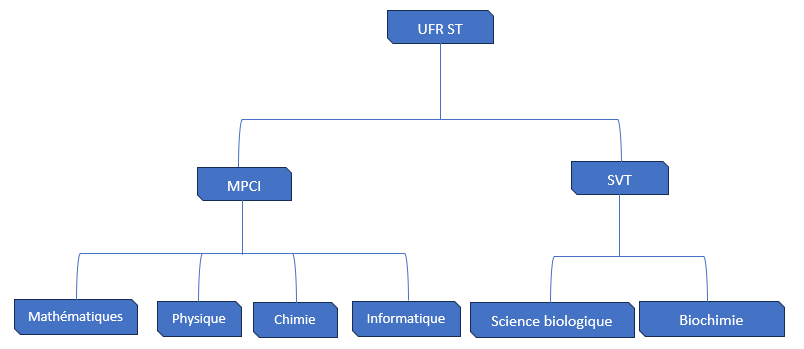
\includegraphics[width=16cm,height=9cm]{images/organigramme st.PNG}%
    }
    \caption{Organigramme des filières de l'UFR ST}%
\end{figure}


\section{Cadre de stage à la direction des services informatique}
Pour mieux nous imprégner du fonctionnement du monde informatique de l’UNZ et pour un apprentissage dans le but de nous faciliter l’insertion dans le milieu professionnel, un stage nous a été accordé pour une durée de trois mois à la DSI dont l’actuel directeur est Mr Paounor SOME. \par

Ce stage nous à permis non seulement de voir de près les équipements informatiques de L’UNZ, mais également d’affuter nos connaissances dans divers domaines de l’informatique et d’\^etre en contact direct avec des enseignants du domaine qui n’hésitaient pas à nous éclairer de temps à autre. 
Ormis ces avantages, Nous avons travaillé dans un cadre propice en ayant à notre disposition tout ce qui etait nécessaire pour bien accomplir notre mission.

\section*{Conclusion}
L'Université Norbert ZONGO actuellement sous la direction du \textbf{Pr Issa Abdou MOUMOULA} est la structure pour laquelle sera conçu la plateforme numérique des thèses et mémoires. 
Pour mener à bien cette tâche, nous avons effectué un stage de trois mois à la direction des services informatique de l'Université.\par 
Dans ce chapitre nous avons présenté l'Université ainsi que ses dirigeants depuis sa création. Aussi nous avons présenté les différentes UFR ainsi que la structure de notre UFR qui est l'UFR-ST.  %Presentation de l'université norbert zongo

\chapter{Contexte, problématique et objectifs}
\markboth{Chapitre 2. Contexte, problématique et objectifs}{} 
\begin{spacing}{1.2}
\minitoc
\thispagestyle{MyStyle}
\end{spacing}
\newpage
\section*{Introduction}
Dans ce chapitre il s'agira pour nous de faire connaitre les fondements de la mise en place de notre plateforme, de faire ressortir la question autour de laquelle gravite notre travail et d'identifier les objectifs que nous nous sommes fixés . \par
\section{Contexte}
La réalisation de notre plateforme numérique s'inscrit dans un contexte où l'accès aux ressources académiques dans les bibliothèques physiques pose de nombreux défis. Hormis de leur richesse, les bibliothèques traditionnelles souffrent souvent de limitations qui entravent l'accès aux informations pour les étudiants et les chercheurs. Parmi ces limitations, on peut citer la disponibilité restreinte des documents, le nombre limité de copies pour des ouvrages particulièrement demandés, et la difficulté à localiser des thèses ou mémoires de qualité et pertinentes.\par
L'accès simultané pour plusieurs personnes à une même ressource est un problème récurrent dans les bibliothèques physiques. Lorsqu'un ouvrage ou une thèse est particulièrement sollicité, les utilisateurs peuvent se retrouver en liste d'attente ou se heurter à l'indisponibilité des documents. Cette situation freine le progrès des recherches et la préparation des travaux académiques.\par
De plus, le manque ou la difficulté à trouver des thèses et mémoires dignes d'intérêt est un autre obstacle majeur. Les utilisateurs doivent souvent consacrer un temps considérable à fouiller parmi des centaines de documents pour identifier ceux qui correspondent le mieux à leurs besoins spécifiques. Ce processus peut être laborieux et décourageant, surtout lorsque les ressources disponibles sont dispersées et mal cataloguées.
\par
\section{Problématique}
Comment surmonter les obstacles liés à l'accès restreint et à la disponibilité limitée des ressources académiques dans les bibliothèques physiques, tout en facilitant la recherche et l'accès simultané aux thèses et mémoires de qualité pour un grand nombre d’utilisateurs ?\par
\section{Objectifs}
Il s'agira pour nous dans cette section de présenter les objectifs fondamentaux d'un tel projet en mettant en lumière son importance dans le contexte de la communauté estudiantine. \par
\subsection{Conservation des thèses et mémoires au format numérique}
La conservation des documents au format numérique représente un tournant majeur dans la gestion et la préservation du patrimoine académique. En optant pour cette approche, la bibliothèque de thèses et mémoires garantit une conservation à long terme des travaux de recherche, tout en offrant une accessibilité accrue aux utilisateurs. Cette transition vers le numérique présente plusieurs avantages significatifs. Elle permettra de :\par

	Préserver l'intégrité des documents dans des conditions optimales. Contrairement aux supports physiques qui sont sujets à la détérioration, à la perte ou au vol, les fichiers numériques peuvent être sauvegardés et stockés de manière sécurisée, réduisant ainsi les risques de perte de données précieuses. De plus, grâce aux technologies de sauvegarde et de stockage en ligne, il est possible de créer des copies de sauvegarde afin de garantir la pérennité des documents, même en cas de sinistre.\par

	Faciliter l’accès pour les utilisateurs. Avec une simple connexion à internet, les étudiants, chercheurs et membres de la communauté académique peuvent consulter et télécharger les documents à tout moment et depuis n'importe quel endroit. Cette facilité d'accès transcende les frontières physiques des bibliothèques traditionnelles, permettant ainsi aux utilisateurs d'explorer un vaste ensemble de ressources documentaires sans contraintes géographiques.\par

	Offrir des fonctionnalités de recherche avancées, facilitant la découverte et l'exploration des documents. Notre plateforme de bibliothèques numériques sera équipée d'outils de recherche sophistiqués, permettant aux utilisateurs de trouver rapidement des documents pertinents en utilisant des mots-clés, des filtres de recherche et d'autres critères de recherche avancés. Cette fonctionnalité de recherche améliorée contribue à optimiser l'efficacité de la recherche académique, en permettant aux utilisateurs de découvrir plus facilement des travaux pertinents dans leur domaine d'intérêt.\par

Notre premier objectif est donc d’assurer la pérennité des documents (résultats des travaux de recherches), faciliter l’accès pour les utilisateurs et offrir des fonctionnalités de recherche avancées. Cette transition vers le numérique représente un pas important vers une gestion plus efficace et une diffusion plus large du savoir académique, contribuant ainsi à l'avancement de la recherche et de l'éducation.
\par

\subsection{Echange entre les auteurs des travaux de recherche et la communauté estudiantine}
Au cœur de la conception de notre plateforme réside un autre objectif primordial, il s'agit de favoriser un échange dynamique et enrichissant entre les auteurs des travaux de recherche et la communauté académique qui les entoure. Cette rubrique se concentre sur la mise en lumière de cet objectif essentiel, soulignant comment notre plateforme aspire à créer un espace d'interaction où les éclaircissements et les discussions entre les auteurs et la communauté peuvent prospérer.

En développant cette plateforme, notre vision est de transcender les frontières traditionnelles de la communication académique en favorisant un dialogue ouvert et transparent. À travers une interface interactive permettant de :\par

	Avoir un espace d’échange où chacun pourra apprécier les travaux ou exposer ses différentes préoccupations afin que les auteurs puissent répondre aux questions, clarifier les points complexes.\par
	Echanger des idées novatrices entre les membres de la communauté universitaire et les auteurs ou même entre auteurs.
	De même, la communauté pourra bénéficier directement des connaissances et des perspectives des auteurs, enrichissant ainsi leur compréhension et leur engagement avec les recherches présentées.\par

En mettant en avant cet objectif central, nous aspirons à créer une plateforme qui transcende les barrières traditionnelles de la recherche académique, favorisant une culture de collaboration, de transparence et d'ouverture. Par cette approche, nous visons à renforcer les liens entre chercheurs et public, à promouvoir une compréhension plus approfondie des travaux de recherche et à catalyser l'innovation et le progrès dans notre communauté universitaire.
\par
Notre second objectif, est de créer un espace d'échange entre les auteurs des travaux de recherche et la communauté académique. En favorisant un dialogue ouvert, transparent et interactif, nous aspirons à créer un environnement propice à la collaboration et à l'enrichissement mutuel des connaissances. À travers cette démarche, nous croyons fermement que notre plateforme contribuera à renforcer les liens au sein de la communauté académique, à promouvoir une culture de partage et d'apprentissage continu, et à catalyser l'avancement de la recherche et de l'innovation.\par
En somme, les objectifs de notre plateforme visent à répondre à un besoin essentiel dans le domaine de la recherche académique : celui de créer un espace dynamique où la numérisation des travaux de recherche et la collaboration entre les auteurs et la communauté universitaire peuvent prospérer. En favorisant la diffusion transparente et accessible et sécurisé des connaissances tout en encourageant les échanges constructifs et la coopération entre les chercheurs et les membres de la communauté, nous aspirons à stimuler l'innovation, à renforcer les liens au sein de la communauté universitaire et à contribuer à l'avancement global de la recherche. Par cette approche intégrée, notre plateforme s'engage à jouer un rôle significatif dans la promotion d'une culture de recherche ouverte, collaborative et tournée vers l'avenir, où le partage du savoir est au cœur de notre mission commune.
\section*{Conclusion}

En conclusion, la mise en place de notre plateforme numérique de thèses et mémoires répond à une nécessité pressante d'améliorer l'accès aux ressources académiques dans un contexte où les bibliothèques physiques présentent de nombreuses limitations. En transformant ces documents en ressources numériques, nous offrons une solution efficace pour surmonter les obstacles liés à la disponibilité restreinte et à l'accès limité aux ouvrages de qualité.\par

Notre démarche s'articule autour de deux objectifs principaux. Le premier est de garantir la conservation à long terme des travaux de recherche tout en facilitant leur accès à un public plus large grâce aux avantages du numérique. Ce passage au format numérique permet non seulement de préserver les documents dans des conditions optimales, mais aussi de les rendre accessibles de partout et à tout moment, tout en intégrant des fonctionnalités de recherche avancées pour optimiser l'efficacité des recherches académiques.\par

Le second objectif vise à favoriser un échange enrichissant entre les auteurs des travaux de recherche et la communauté universitaire. En créant un espace interactif sur notre plateforme, nous encourageons un dialogue ouvert et constructif, permettant aux utilisateurs de poser des questions, d'obtenir des clarifications et d'échanger des idées novatrices. Ce cadre interactif promeut une culture de collaboration et de transparence, essentielle pour le progrès et l'innovation au sein de la communauté académique.\par

Ainsi, notre plateforme aspire à transcender les barrières traditionnelles de la recherche académique, en offrant une solution numérique intégrée qui répond aux besoins de conservation, d'accès et de collaboration.\par%contexte problematique objectifs et  Methodologie de travail
    
    \doublespacing{}% Double spacing between lines
    \addtocontents{toc}{\protect\setcounter{tocdepth}{2}}
    
    %\chapter{Méthodologie de travail}
\markboth{Chapitre 3. Méthodologie de travail}{} 
\begin{spacing}{1.2}
\minitoc
\thispagestyle{MyStyle}
\end{spacing}
\newpage

\section*{Introduction}
Créer une plateforme est un défi complexe qui nécessite une approche méthodique et efficace. Dans cette optique, nous avons adopté une méthodologie de gestion de projet dénommé Scrum. Cette méthodologie favorise la flexibilité, la collaboration et la livraison continue de fonctionnalités. Au cœur de notre approche réside une méthode itérative et incrémentale qui nous permet de répondre aux besoins évolutifs de notre projet tout en garantissant un développement rapide et efficace.\par

Dans ce chapitre, nous plongerons au cœur de notre méthodologie de travail, détaillant les principes directeurs, les processus et les pratiques adopté pour mener à bien la création de notre plateforme de bibliothèque numérique. En présentant notre méthodologie de manière détaillée, nous visons à offrir un aperçu complet de notre processus de développement, mettant en lumière les stratégies que nous avons adoptées pour assurer le succès de notre projet.
\par
\section{Présentation de la méthodologie agile Scrum}
La méthodologie Agile Scrum est une approche de gestion de projet qui vise à favoriser la flexibilité, la réactivité et la collaboration dans le développement de produits logiciels et de solutions complexes. Contrairement aux méthodologies traditionnelles, Scrum privilégie une approche itérative et incrémentale, où le travail est organisé en cycles courts appelés "sprints"[biblio].
	Au cœur de cette méthodologie se trouvent trois principaux acteurs dont nous endosserons le rôle : le Product Owner, l'Équipe de développement et le Scrum Master. Le Product Owner est chargé de définir les objectifs du projet et de prioriser les fonctionnalités à développer, en se basant sur les besoins du client et les retours utilisateurs. L'Équipe de développement est responsable de la réalisation des tâches et de la livraison des fonctionnalités lors de chaque sprint. Le Scrum Master, quant à lui, est garant du respect des principes Scrum, il facilite les interactions au sein de l'équipe et veille à ce que les processus Scrum soient bien compris et suivis.
La méthodologie Scrum repose également sur un ensemble d'artefacts et d'événements clés. Les principaux artefacts incluent le Product Backlog, qui recense toutes les fonctionnalités à développer, et le Sprint Backlog, qui contient les tâches à réaliser lors de chaque sprint. Les événements Scrum comprennent la Planification du Sprint, qui définit les objectifs du sprint, le Daily Scrum, une réunion quotidienne pour synchroniser le travail de l'équipe, la Revue de Sprint, où les fonctionnalités développées sont présentées au Product Owner, et la Rétrospective de Sprint, qui permet à l'équipe de réfléchir et de s'améliorer continuellement.
En résumé, la méthodologie Agile Scrum offre une approche structurée et adaptable pour gérer efficacement les projets complexes. En favorisant la maneabilité, et la livraison continue de valeur, Scrum permet au développeur d'organiser et de générer plus facilement les tâches à travers des solutions adaptatives pour des problèmes complexes \cite{schwaber2011scrum}.
	
	\begin{figure}[H]%
    \center%
    \setlength{\fboxsep}{5pt}%
    \setlength{\fboxrule}{0.5pt}%
    \fbox{
    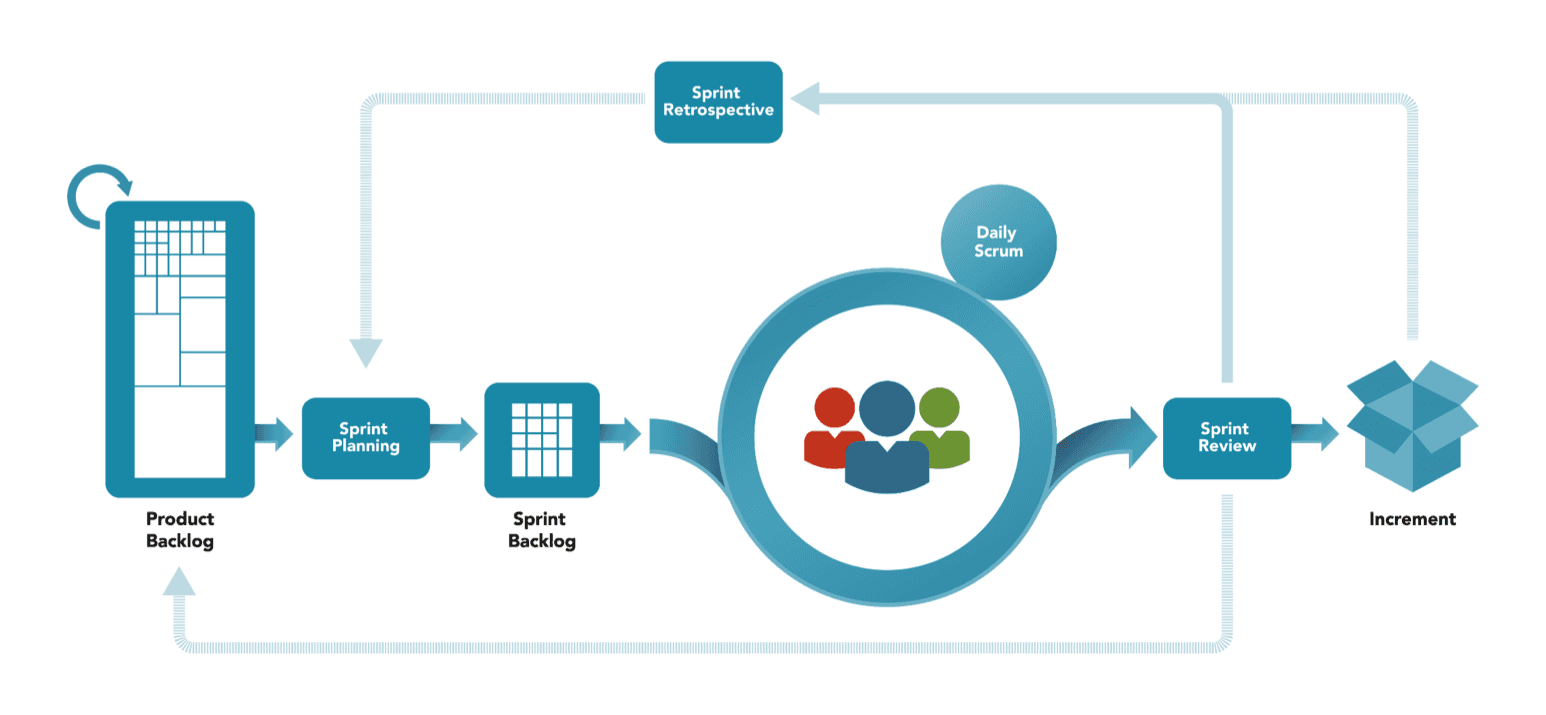
\includegraphics[width=12.5cm,height=9cm]{images/scrum.png}%
    }
    \caption{Fonctionnement de la méthodologie agile scrum}%
\end{figure} \par

\section*{Conclusion}

En adoptant la méthodologie Scrum, notre objectif a été de créer un environnement de travail agile où l'adaptabilité, la transparence et la communication étaient au cœur de notre processus de développement. En nous appuyant sur les valeurs de Scrum telles que le respect, l'engagement et le courage, nous avons relevé avec succès les défis complexes de notre projet tout en restant alignés sur nos objectifs.
À mesure que nous avons avancé dans notre projet, la méthodologie Agile Scrum nous a permis de livrer rapidement des fonctionnalités utilisables et de répondre de manière proactive aux besoins changeants de notre marché. En embrassant les principes de Scrum, nous sommes resté confiants dans notre capacité à créer une plateforme de bibliothèque numérique innovante, robuste et adaptée aux besoins de notre communauté d'utilisateurs.
\par % Methodologie de travail
    
    %\chapter{Méthodologie de travail}
\markboth{Chapitre 3. Méthodologie de travail}{} 
\begin{spacing}{1.2}
\minitoc
\thispagestyle{MyStyle}
\end{spacing}
\newpage

\section*{Introduction}
Créer une plateforme est un défi complexe qui nécessite une approche méthodique et efficace. Dans cette optique, nous avons adopté une méthodologie de gestion de projet dénommé Scrum. Cette méthodologie favorise la flexibilité, la collaboration et la livraison continue de fonctionnalités. Au cœur de notre approche réside une méthode itérative et incrémentale qui nous permet de répondre aux besoins évolutifs de notre projet tout en garantissant un développement rapide et efficace.\par

Dans ce chapitre, nous plongerons au cœur de notre méthodologie de travail, détaillant les principes directeurs, les processus et les pratiques adopté pour mener à bien la création de notre plateforme de bibliothèque numérique. En présentant notre méthodologie de manière détaillée, nous visons à offrir un aperçu complet de notre processus de développement, mettant en lumière les stratégies que nous avons adoptées pour assurer le succès de notre projet.
\par
\section{Présentation de la méthodologie agile Scrum}
La méthodologie Agile Scrum est une approche de gestion de projet qui vise à favoriser la flexibilité, la réactivité et la collaboration dans le développement de produits logiciels et de solutions complexes. Contrairement aux méthodologies traditionnelles, Scrum privilégie une approche itérative et incrémentale, où le travail est organisé en cycles courts appelés "sprints"[biblio].
	Au cœur de cette méthodologie se trouvent trois principaux acteurs dont nous endosserons le rôle : le Product Owner, l'Équipe de développement et le Scrum Master. Le Product Owner est chargé de définir les objectifs du projet et de prioriser les fonctionnalités à développer, en se basant sur les besoins du client et les retours utilisateurs. L'Équipe de développement est responsable de la réalisation des tâches et de la livraison des fonctionnalités lors de chaque sprint. Le Scrum Master, quant à lui, est garant du respect des principes Scrum, il facilite les interactions au sein de l'équipe et veille à ce que les processus Scrum soient bien compris et suivis.
La méthodologie Scrum repose également sur un ensemble d'artefacts et d'événements clés. Les principaux artefacts incluent le Product Backlog, qui recense toutes les fonctionnalités à développer, et le Sprint Backlog, qui contient les tâches à réaliser lors de chaque sprint. Les événements Scrum comprennent la Planification du Sprint, qui définit les objectifs du sprint, le Daily Scrum, une réunion quotidienne pour synchroniser le travail de l'équipe, la Revue de Sprint, où les fonctionnalités développées sont présentées au Product Owner, et la Rétrospective de Sprint, qui permet à l'équipe de réfléchir et de s'améliorer continuellement.
En résumé, la méthodologie Agile Scrum offre une approche structurée et adaptable pour gérer efficacement les projets complexes. En favorisant la maneabilité, et la livraison continue de valeur, Scrum permet au développeur d'organiser et de générer plus facilement les tâches à travers des solutions adaptatives pour des problèmes complexes \cite{schwaber2011scrum}.
	
	\begin{figure}[H]%
    \center%
    \setlength{\fboxsep}{5pt}%
    \setlength{\fboxrule}{0.5pt}%
    \fbox{
    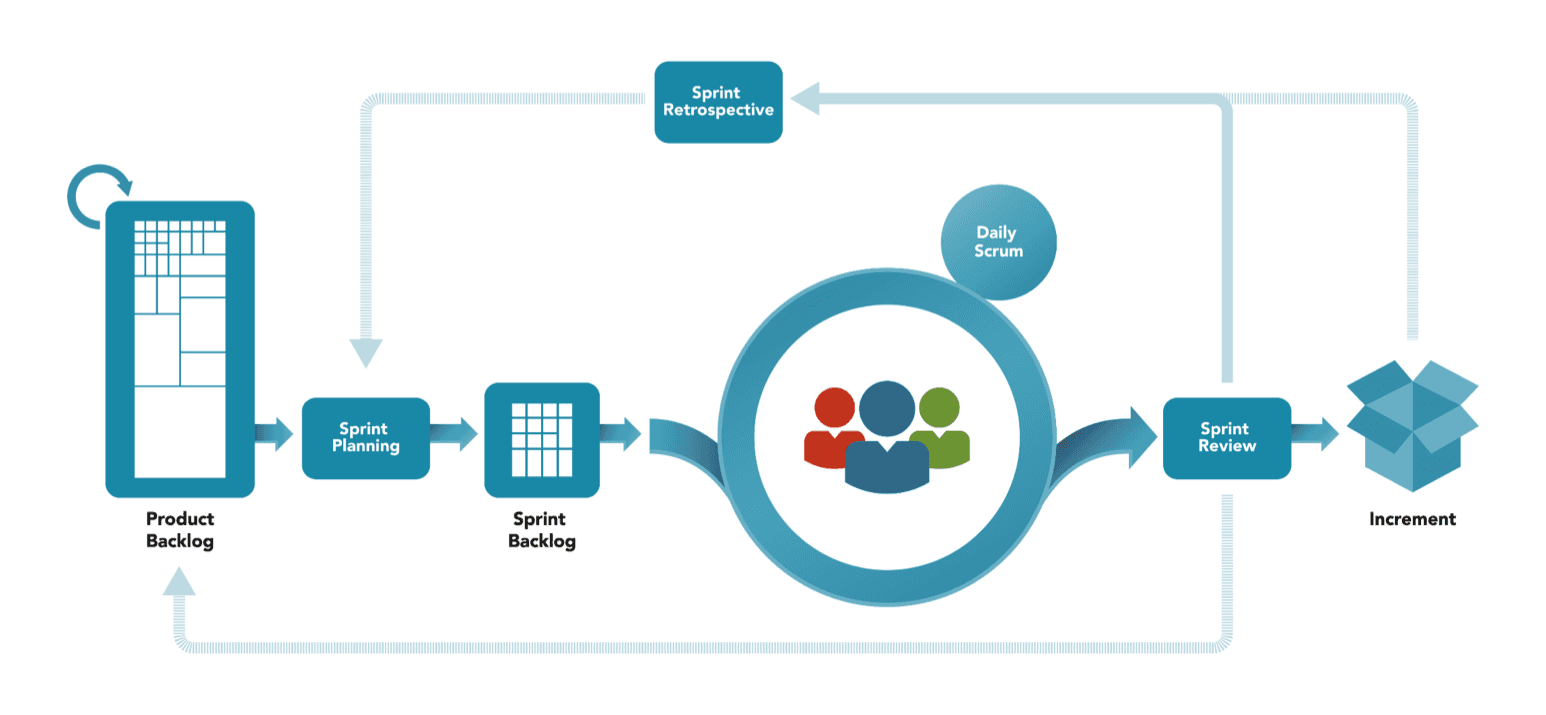
\includegraphics[width=12.5cm,height=9cm]{images/scrum.png}%
    }
    \caption{Fonctionnement de la méthodologie agile scrum}%
\end{figure} \par

\section*{Conclusion}

En adoptant la méthodologie Scrum, notre objectif a été de créer un environnement de travail agile où l'adaptabilité, la transparence et la communication étaient au cœur de notre processus de développement. En nous appuyant sur les valeurs de Scrum telles que le respect, l'engagement et le courage, nous avons relevé avec succès les défis complexes de notre projet tout en restant alignés sur nos objectifs.
À mesure que nous avons avancé dans notre projet, la méthodologie Agile Scrum nous a permis de livrer rapidement des fonctionnalités utilisables et de répondre de manière proactive aux besoins changeants de notre marché. En embrassant les principes de Scrum, nous sommes resté confiants dans notre capacité à créer une plateforme de bibliothèque numérique innovante, robuste et adaptée aux besoins de notre communauté d'utilisateurs.
\par%Etude conceptuelle
    
    \chapter{Etude conceptuelle}
\markboth{Chapitre 4. Etude conceptuelle}{} 
\begin{spacing}{1.2}
\minitoc
\thispagestyle{MyStyle}
\end{spacing}
\newpage

\section*{Introduction}
Le chapitre suivant marque une étape cruciale dans le processus de développement de notre plateforme de bibliothèque numérique. Cette phase englobe plusieurs aspects essentiels, notamment l'étude de l'existant, la définition précise des fonctionnalités attendues et la création d'un dictionnaire des données pour structurer les informations manipulées par la plateforme et les diagrammes de classe.\par
Dans ce chapitre, nous explorerons en détail chacun de ces éléments, en mettant en lumière leur importance dans la conception de notre plateforme.\par

Dans l'ensemble, ce chapitre constitue une étape fondamentale dans le processus de développement de notre plateforme de bibliothèque numérique. En explorant l'existant, la définition des fonctionnalités la création du dictionnaire des données et la mise en place des diagrammes de classe, nous jetterons les bases d'une conception solide et fonctionnelle, garantissant ainsi le succès de notre projet.
\par
\section{Etude de l'existant}
L'étude de l'existant permet au développeur de s'imprégner du fonctionnement et de recueillir les informations nécessaire du système actuel (ancien système) pour avoir une vision du futur système(système à concevoir).\par
Dans notre cas, l'étude de l'existant nous a permis de de faire ressortir les fonctionnalités qui seront greffé à notre bibliothèque ainsi que les information nécessaire à sa mise en place et son bon fonctionnement.

\subsection{Définition des Fonctionnalités }
La définition des fonctionnalités de notre plateforme de bibliothèque numérique constitue une étape importante dans notre processus de développement. Ces fonctionnalités sont conçues pour répondre aux attentes et pour offrir une expérience utilisateur fluide et efficace. Parmi les fonctionnalités clés que nous avons identifiées, nous pouvons citer :

\paragraph{Mise en ligne de document : Les utilisateurs ont la possibilité de mettre en ligne leurs documents, tels que des thèses, des mémoires ou des articles de recherche, sur la plateforme. Cette fonctionnalité intuitive et conviviale permet aux auteurs de partager leurs travaux avec la communauté académique de manière simple et efficace.}


\paragraph{Validation de la mise en ligne : Avant la publication définitive sur la plateforme, les documents soumis font l'objet d'une validation par un administrateur désigné. Cette étape de validation garantit la qualité et la pertinence des documents publiés, tout en assurant le respect des normes et éthiques.}

\paragraph{Recherche de document avec mots-clés : Les utilisateurs peuvent effectuer des recherches avancées sur la plateforme en utilisant des mots-clés spécifiques. Cette fonctionnalité permet une exploration efficace de la base de données, en permettant aux utilisateurs de trouver rapidement des documents pertinents dans leur domaine d'intérêt.}


\paragraph{
Publication de préoccupations : Les utilisateurs ont la possibilité de publier des préoccupations ou des questions relatives aux documents disponibles sur la plateforme. Cette fonctionnalité encourage l'interaction et la collaboration entre les membres de la communauté académique, en permettant aux utilisateurs de partager leurs réflexions et leurs interrogations avec leurs pairs.}

\subsection{Dictionnaire des données}
Le dictionnaire des données constitue la pierre angulaire de la structure de notre plateforme de bibliothèque numérique. Il offre une vue exhaustive et organisée des entités, des attributs et des relations qui composent notre système, fournissant ainsi un cadre solide pour la gestion et l'exploitation des données.\par

Les attributs dont nous avons fait usage dans la mise en place de notre plateforme ainsi que leurs description et typage sont consignés dans le tableau ci-dessous.
\par 

 Utilisateur  :
\renewcommand{\labelitemi}{\tiny$\bullet$}
\begin{itemize}[leftmargin=2cm, topsep=0pt]
        \begin{spacing}{1.25}
        \item Description : Cette entité représente les utilisateurs de la plateforme, comprenant les auteurs, les lecteurs et les administrateurs.
        \item Attributs :
        \begin{itemize}[leftmargin=2cm, topsep=0pt]
        \begin{spacing}{1.25}
        \item 	Identifiant utilisateur (ID) de type 			entier
        \item item2
        \item item3
        \end{spacing}
\end{itemize}
        \item item3
        \end{spacing}
\end{itemize}
\begin{spacing}{0.5}
\end{spacing}

\subsection{Diagrammes de classe}
Les diagrammes de classe ont fait partie intégrante de la modélisation orientée objet et ont permis de visualiser la structure statique du système en définissant les classes, leurs attributs, leurs méthodes ainsi que les relations entre elles.\par

Ces diagrammes nous ont offert une représentation claire et structurée de notre système, facilitant ainsi la compréhension des différentes composantes et de leurs interactions. En établissant un modèle précis, nous avons pu identifier les éléments clés et leurs connexions, ce qui a aidé à garantir la cohérence et la robustesse de l'architecture de notre application.\par

Dans cette section, nous détaillons les différents diagrammes de classe élaborés pour notre projet. Chaque diagramme est accompagné d'une explication des classes principales, des associations et des dépendances, mettant en lumière les fonctionnalités et les comportements de notre plateforme. L'objectif a été de fournir une vue d'ensemble complète et détaillée qui serve de guide pour la phase de développement et assure une base solide pour les futures extensions et maintenances du système.\par

	\begin{figure}[H]%
    \center%
    \setlength{\fboxsep}{5pt}%
    \setlength{\fboxrule}{0.5pt}%
    \fbox{
    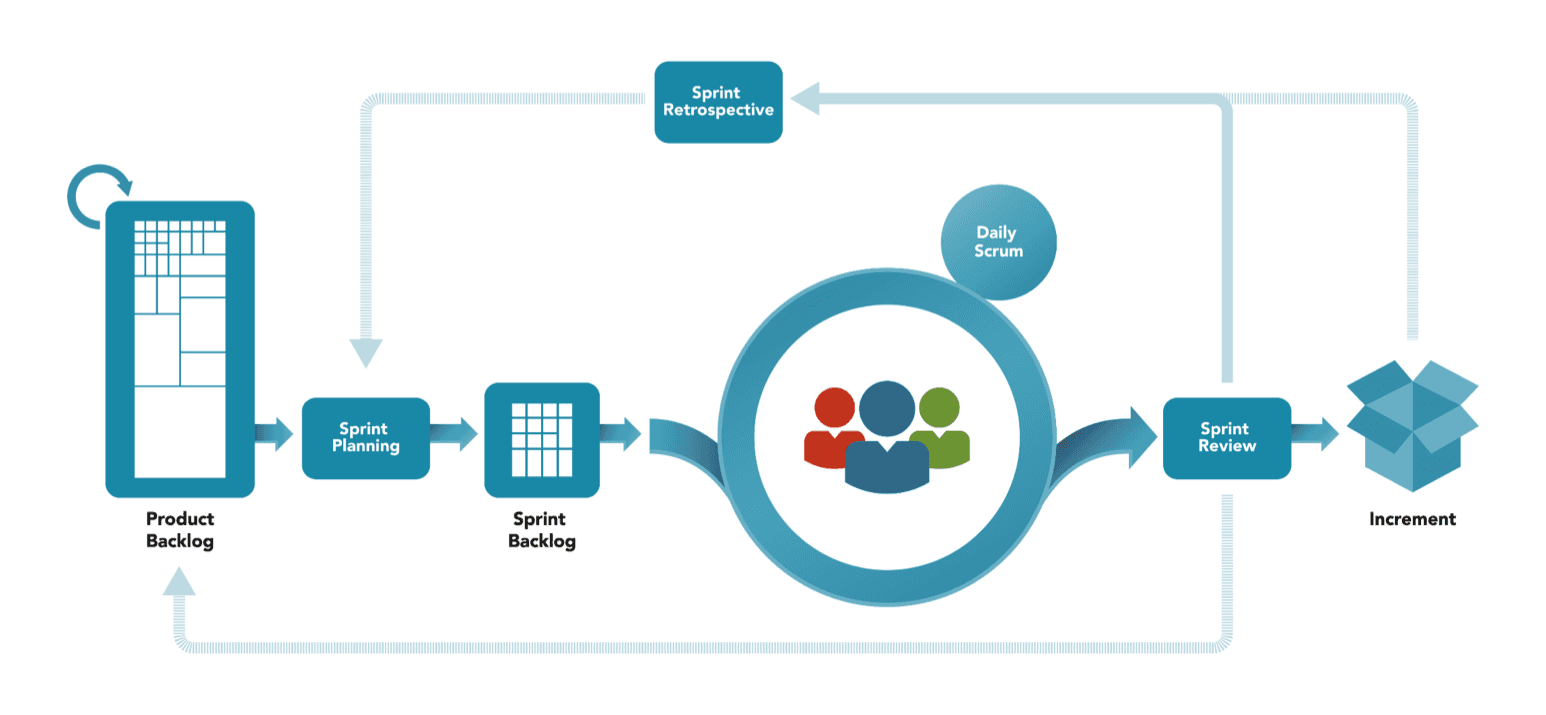
\includegraphics[width=12.5cm,height=9cm]{images/scrum.png}%
    }
    \caption{Fonctionnement de la méthodologie agile scrum}%
\end{figure} \par

\subsection{Règles de gestion}
Pour atteindre nos objectifs nous avons intégré dans notre système un certains nombre de règle pour un bon traitement des information. Ces règles sont les suivantes:
\renewcommand{\labelitemi}{\tiny$\bullet$}
\begin{itemize}[leftmargin=2cm, topsep=0pt]
        \begin{spacing}{1.25}
        
        \item Chaque UFR regroupe un ensemble de document.
        \item Chaque document est associé à un ou auteur.
        \item Chaque préoccupation est associée à un document spécifique.
        \item Chaque réponse est associée à une préoccupation correspondante.
        \end{spacing}
\end{itemize}
\begin{spacing}{0.5}
\end{spacing}

%Etude conceptuelle    
    
     \chapter{Implémentation et concrétisation}
\markboth{Chapitre 4. Implementation et concrétisation}{} 
\begin{spacing}{1.2}
\minitoc
\thispagestyle{MyStyle}
\end{spacing}
\newpage

\section*{Introduction}
Dans cette phase de développement de notre plateforme de bibliothèque numérique, nous avons été confrontés à une grande responsabilité : transformer nos plans en réalité. Ce chapitre marque ainsi le passage de la planification à la concrétisation de notre projet.\par
    La première étape a consisté à choisir les outils et les technologies les plus adaptés à notre projet. Cette décision a été cruciale, car elle a influencé la manière dont nous avons conçu et mis en œuvre les fonctionnalités de notre application. Nous avons exploré les critères pris en compte dans ce choix, ainsi que les avantages et les inconvénients des différentes options disponibles.
    Ensuite, nous avons abordé la création des modèles et la migration vers la base de données. Cette phase a été fondamentale dans la construction de notre plateforme, car elle a impliqué la conception des structures de données et des relations entre les entités, ainsi que la migration des données existantes vers la nouvelle architecture.
     Enfin, nous nous sommes plongés dans le développement des fonctionnalités de notre plateforme, où chaque ligne de code que nous avons écrite a contribué à donner vie à notre vision. Nous allons détailler les différentes fonctionnalités que nous avons développées.
   En résumé, ce chapitre met en lumière notre rôle de développeur dans la réalisation de notre plateforme de bibliothèque numérique. Nous détaillerons les différentes phases d'implémentation et les défis rencontrés tout au long du processus.

\section{Choix des outils}
Dans cette section, nous abordons le choix des outils pour le développement de notre plateforme de bibliothèque numérique, Une étape importante dans la concrétisation de notre projet car les outils sélectionnés ont eu un impact significatif sur la manière dont nous avons conçu et mis en œuvre les fonctionnalités de notre plateforme.\par

Nous avons pris soin d'analyser les différentes options disponibles, en tenant compte de divers critères tels que la facilité d'utilisation, la compatibilité avec nos besoins, la robustesse et la popularité dans la communauté de développement. Notre objectif était de choisir des outils qui nous permettraient de maximiser notre productivité tout en garantissant la qualité et la fiabilité de notre plateforme.\par

Nous détaillerons les processus de sélection des outils, en mettant en lumière les critères et les considérations qui ont guidé nos choix. Nous examinerons également les outils spécifiques que nous avons finalement sélectionnés pour chaque aspect du développement de notre plateforme, ainsi que les raisons derrière ces choix. Enfin, nous discuterons des avantages et des défis associés à l'utilisation de ces outils dans le contexte de notre projet.\par

En résumé, ce chapitre offre un aperçu détaillé du processus de sélection des outils pour le développement de notre plateforme de bibliothèque numérique, mettant en évidence les décisions prises et les implications de ces choix sur le déroulement et les résultats de notre projet.

\subsection{Environnement de développement intégré (IDE)}
L'un des premiers éléments que nous avons abordés est l'environnement de développement intégré (IDE), qui constitue un pilier essentiel de notre workflow de développement.\par

	Comme définition, un environnement de développement intégré (IDE) est un logiciel qui fournit un ensemble complet d'outils pour les développeurs afin de faciliter la création, la modification, le débogage et le déploiement de logiciels. En d'autres termes, un IDE est un environnement logiciel unifié qui regroupe plusieurs fonctionnalités essentielles pour le développement de logiciels dans une seule interface utilisateur.\par 

Les IDE sont conçus pour offrir une expérience de développement intégrée et fluide, en fournissant des fonctionnalités telles que :\\

	Éditeur de code : Un éditeur de code intégré permet aux développeurs d'écrire, de modifier et de formater du code source dans divers langages de programmation. Cet éditeur offre souvent des fonctionnalités avancées telles que la coloration syntaxique, l'autocomplétions, l'indentation automatique et la mise en évidence des erreurs de syntaxe.
\par
	Outils de débogage : Les IDE fournissent des outils de débogage puissants qui permettent aux développeurs d'identifier et de corriger les erreurs dans leur code. Ces outils permettent de mettre en pause l'exécution du programme, d'inspecter les variables, de suivre l'exécution du code ligne par ligne et de détecter les erreurs de logique.\par

	Gestion de projet : Les IDE offrent des fonctionnalités de gestion de projet qui permettent aux développeurs d'organiser et de gérer efficacement leur code source, leurs fichiers et leurs ressources. Cela inclut souvent des fonctionnalités telles que la navigation dans le code, la recherche de fichiers, la gestion des dépendances et la gestion de versions.\par

	Intégration avec des outils externes : Les IDE intègrent souvent des outils externes tels que des compilateurs, des gestionnaires de packages, des outils de contrôle de version et des environnements de test, ce qui permet aux développeurs d'accéder à toutes les fonctionnalités dont ils ont besoin à partir d'une seule interface.\par

En somme, un IDE est un outil essentiel pour les développeurs de logiciels, car il leur fournit un environnement de développement unifié et complet qui simplifie et accélère le processus de création de logiciels. Grâce à ses fonctionnalités avancées, un IDE permet aux développeurs de travailler de manière plus efficace et productive, en leur offrant les outils nécessaires pour créer des applications de haute qualité.\par

Concernant notre projet nous avons opté pour Visual Studio Code (VS Code), un environnement polyvalent et puissant qui a grandement facilité notre travail tout au long du projet.
Dans cette section, nous détaillerons notre choix d'utiliser VS Code comme IDE principal pour le développement de notre plateforme. Nous explorerons les raisons derrière ce choix, en mettant en lumière les fonctionnalités clés et les extensions de VS Code que nous avons utilisés pour améliorer notre flux de travail et pour personnaliser notre environnement de développement en fonction de nos besoins spécifiques. Nous préciserons comment ces extensions ont optimisé notre productivité et nous ont permis de gérer efficacement les tâches de développement complexes.
En résumé, ce chapitre offre un aperçu détaillé de notre utilisation de Visual Studio Code comme IDE principal pour le développement de notre plateforme de bibliothèque numérique. \par 

\begin{figure}[H]%
    \center%
    \setlength{\fboxsep}{5pt}%
    \setlength{\fboxrule}{0.5pt}%
    \fbox{
    
\includegraphics[width=4cm,height=4cm]{images/vs code.jpg}%
    }
    \caption{Logo de VS Code}%
\end{figure}

Dans le tableau suivant, nous avons consigné les fonctionnalité et extensions de VS Code dont nous avons fait usage.
\begin{table}[h!]
    \centering
    \begin{tabular}{|p{4cm}|p{9cm}|}
        \hline
        Fonctionnalité/extension & Rôle \\
        \hline
        Terminal & Fonctionnalité permettant l'utilisation d'un terminal \\
        \hline
        Emmet & Fonctionnalité permettant l’autocomplétions et la génération de code en HTML \\
        \hline
        CSS formatter & Extension pour le formatage de code CSS \\ \hline
       HTML CSS Support & Extension pour l’autocomplétions de code CSS directement dans du code HTML \\ \hline
     Laravel Intelephense & Extension pour:
\renewcommand{\labelitemi}{\tiny$-$}
\begin{itemize}[leftmargin=2cm, topsep=0pt]
        
        \item voir les suggestions de code Laravel
        \item faire l’autocomplétions de code Laravel
        \item Gérer les importation
        
\end{itemize} 
 \\ \hline
 
      Laravel Snippets  & Extension pour l’autocomplétions  lors de la création des routes.\\ \hline
      Laravel goto view & Extension pour passer d’un Controller à une vue blade grâce au nom de la vue \\ \hline
     Laravel Blade Snippets & Extension pour:
\renewcommand{\labelitemi}{\tiny$-$}
\begin{itemize}[leftmargin=2cm, topsep=0pt]
        
        \item la coloration syntaxique dans les vues Blade
        \item Génération de code incluant des balises HTML et des directives blade
        \item l’utilisation de l’extension Emmet dans les vues blade
       
\end{itemize}
 \\ \hline
     Laravel Blade formatter & Extension pour l’autocomplétions de code dans les vues blade \\ \hline
     Codeium & Fonctionnalité pour l’utilisation d’intelligence artificielle pour la génération et le débogage de code dans vs code.\\ \hline
        \hline
    \end{tabular}
    \caption{Quelques extension de VS Code et leur rôle}
    \label{Tableau:Quelques extensions de VS Code et leur rôle}
\end{table}
\par
 Outre ces fonctionnalités, notre choix de VS Code se justifie par le fait qu'il s'agit d'un IDE très populaire\cite{code2019visual}. De plus, nous nous sommes familiarisés avec VS Code depuis un certain temps. Nous avons donc trouvé judicieux d’opter pour cet éditeur, ce qui s’est avéré être un bon choix, car nous n’avons pas eu de difficulté à trouver de l’aide lorsque nous avons rencontré des problèmes et nous avons travaillé sur un interface qui nous était familière. 
\par

Le choix de VS Code nous a été d’un avantage considérable, car il a grandement facilité l'implémentation et la structuration de notre projet. Grâce à son interface conviviale et à ses nombreuses fonctionnalités, nous avons pu travailler de manière plus efficace et organisée. Néanmoins, nous avons rencontré quelques difficultés, notamment avec certaines extensions qui, à l'occasion, cessaient de fonctionner correctement. Il nous fallait alors les désactiver et les réactiver périodiquement pour résoudre ces problèmes. Malgré ces inconvénients mineurs, l'utilisation de VS Code s'est avérée globalement bénéfique pour notre travail.
\par 


\subsection{Serveur local}
Un serveur local est un environnement de serveur web installé directement sur un ordinateur personnel ou une machine de développement. Il simule les conditions d'un serveur en ligne, permettant aux développeurs de créer, tester et modifier des applications web en toute sécurité avant de les déployer en production. L'utilisation d'un serveur local est essentielle dans le développement de projets web, car elle permet de tester et d'affiner les fonctionnalités avant de les déployer en production. Un serveur local offre un environnement sécurisé et contrôlé, où les développeurs peuvent expérimenter, corriger les erreurs et optimiser le code sans impact sur les utilisateurs finaux.

Pour le développement de notre projet, nous avons opté pour l'utilisation de Laragon comme serveur local. Laragon est une plateforme de développement rapide et puissante qui facilite la gestion d'environnements de développement web. Elle est conçue pour être légère, portable, et rapide, offrant une alternative efficace aux autres solutions telles que XAMPP ou WAMP.

Laragon se distingue par sa simplicité d'installation et de configuration. En quelques clics, il permet de mettre en place un environnement de développement complet, incluant Apache, MySQL, PHP [biblio], et bien d'autres outils indispensables. De plus, Laragon prend en charge les dernières versions de ces logiciels [biblio], garantissant ainsi que notre environnement de développement reste à jour avec les technologies actuelles.


En utilisant Laragon, nous avons pu optimiser notre flux de travail et améliorer notre productivité. Ses performances élevées et sa stabilité ont permis de réduire les temps de chargement et d'exécution, tout en offrant un environnement cohérent et fiable. De plus, 
Laragon est un environnement de développement universel portable, isolé, rapide et puissant pour PHP, Node.js, Python, Java, Go, Ruby. Il est rapide, léger, facile à utiliser et facile à étendre \cite{laragon.org}.

En résumé, Laragon s'est révélé être un choix judicieux pour notre serveur local, grâce à sa facilité d'utilisation, ses performances remarquables et sa flexibilité. Il a joué un rôle crucial dans le succès du développement de notre bibliothèque numérique de thèses et mémoires, en nous fournissant une base solide et fiable pour construire et tester notre plateforme.

\subsection{Système de gestion de version}
Un autre outil crucial dans notre processus de développement a été le système de gestion de version, plus précisément Git. L'utilisation d'un VCS (Version Control System) est indispensable pour tout projet de développement, car il permet de gérer les modifications apportées au code source au fil du temps, facilitant ainsi, la gestion des versions et le suivi des changements \cite{loeliger2012version}.
\par 

Comme définition, un système de gestion de version est un logiciel qui aide les développeurs à suivre les modifications du code source, à collaborer avec d'autres développeurs et à maintenir un historique complet des changements \cite{zolkifli2018version}. Git, en particulier, est un VCS distribué, ce qui signifie que chaque développeur possède une copie complète de l'historique du projet, facilitant le travail hors ligne et améliorant la résilience du projet.


Fonctionnalités clés de Git nous ayant servi: \\
\par 
Suivi des Modifications : Git enregistre chaque modification apportée aux fichiers, permettant de suivre l'historique des changements.Il facilite également la comparaison entre différentes versions du code source, rendant plus simple l'identification des différences et des modifications spécifiques.
\par 
Branches et Fusions : Git permet de créer des branches pour développer des fonctionnalités ou corriger des \index{bugs}bugs indépendamment de la branche principale. 
Les outils de fusion de Git sont puissants et permettent de combiner les changements de différentes branches de manière fluide et efficace.
\par 
Réversibilité: En cas de problème, Git permet de revenir facilement à une version précédente, assurant la sécurité et la stabilité du projet.
Cette capacité à annuler les modifications nous a été cruciale pour le développement de plateforme.
\par 
En conclusion, Git a joué un rôle central en tant que système de gestion de version. Même en tant que développeur unique. Ce fut un outil indispensable pour assurer une gestion efficace et organisée de notre code source. Son utilisation nous a permis de développer notre plateforme de manière structurée, sécurisée et flexible.

\subsection{Plateforme de Gestion de Version}
En complément de Git, nous avons utilisé une plateforme de gestion de version et de collaboration pour pouvoir gérer le suivi des modifications de code, la gestion de projets, et la collaboration entre développeurs bien que notre projet ait été réalisé par un seul développeur. Nous avons opté pour GitHub qui est le plus populaire avec plus de 3,5 million d'utilisateurs \cite{lima2014coding} en 2013.
GitHub nous a fourni des avantages significatifs pour la gestion et l'organisation du code tel que :
Les Dépôts (Repositories) : GitHub permet de créer des dépôts (repositories) pour héberger le code source. Chaque dépôt contient l'historique complet des modifications et les branches du projet. Les dépôts peuvent être publics ou privés, offrant ainsi une flexibilité en termes de visibilité et de collaboration au besoin. \par
Gestion centralisée du code : Les dépôts GitHub permettent de stocker le code source de manière centralisée, offrant un accès sécurisé et structuré à toutes les versions du code. Cette centralisation facilite la gestion des différentes branches et versions du projet, même pour un développeur unique.
\par Pour notre projet, GitHub a hébergé notre dépôt de code, offrant un accès centralisé et sécurisé à l'historique complet des modifications et aux différentes branches. Cette centralisation a facilité la gestion des versions, la sauvegarde du code et la restauration en cas de besoin. Aussi, en utilisant GitHub, nous avons pu suivre les modifications apportées au code de manière systématique, facilitant le retour à des versions antérieures si nécessaire. Le stockage du code sur GitHub a assuré une sauvegarde fiable et un accès constant, ce qui est crucial pour éviter la perte de données et pour travailler de manière flexible depuis n'importe quel endroit. 
\par
En conclusion, GitHub a été un outil indispensable pour la gestion et l'organisation de notre projet. Sa fonctionnalité de gestion centralisée du code a permis de maintenir une approche méthodique et efficace, assurant la qualité et la stabilité de notre plateforme numérique. Grâce à GitHub, nous avons pu gérer notre code source de manière structurée, sécurisée et accessible.

\section{Choix des technologies}
Après avoir achevé les différentes étapes de conception, nous avons entamé la concrétisation de notre projet en utilisant un ensemble de technologies complémentaires. Pour structurer le contenu de notre application, nous avons utilisé le langage de balisage HTML. La présentation et le style ont été assurés par CSS. En ce qui concerne les \index{langages de programmation}langages de programmation , nous avons principalement utilisé PHP avec son framework Laravel, et JavaScript accompagné de la bibliothèque JQuery pour ajouter des fonctionnalités dynamiques et interactives. \par 

Ce chapitre dévoilera en détail la conception de notre plateforme, en présentant les architectures mises en place. Nous explorerons comment chaque technologie a été intégrée pour répondre aux besoins spécifiques de notre projet. En un mot, nous exposerons les rouages internes de notre application, y compris les structures de base de données, les interfaces utilisateur, et les fonctionnalités principales, afin de donner une vision complète et transparente de son fonctionnement.

\subsection{HTML5}
HTML (HyperText Markup Language) est la structure de base dans toute les pages web \cite{lubbers2011pro}.
Son utilisation a permis de créer une structure de page claire, sémantique et \index{accessible}accessible, posant ainsi les bases solides pour une expérience utilisateur optimale. HTML5 a été le premier pas vers la réalisation de notre plateforme, garantissant que chaque page est bien organisée et facile à naviguer.
HTML5 a donc servir à mettre en place le squelette de notre plateforme.


\begin{figure}[H]%
    \center%
    \setlength{\fboxsep}{5pt}%
    \setlength{\fboxrule}{0.5pt}%
    \fbox{
    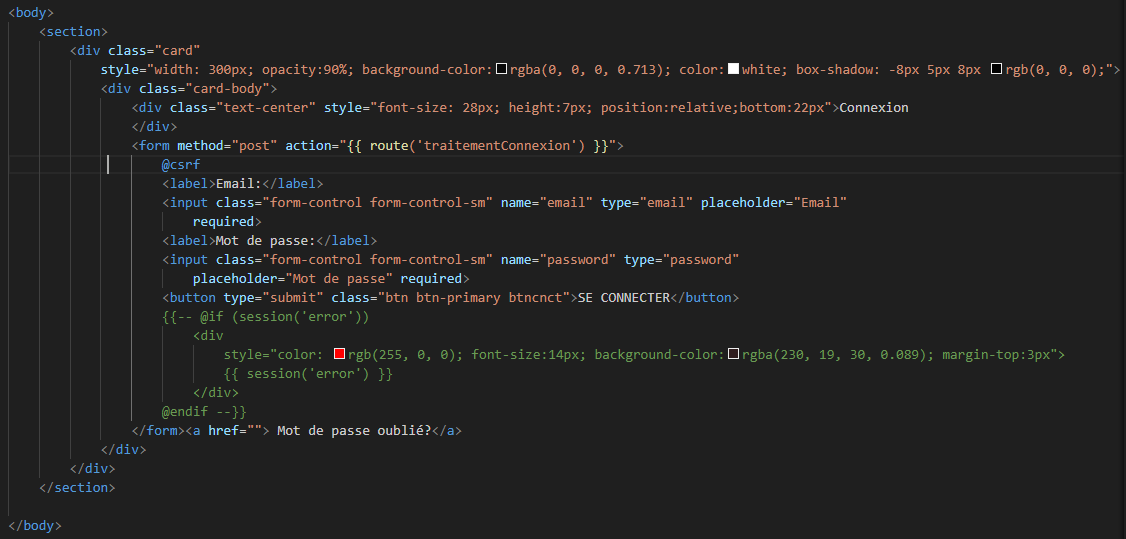
\includegraphics[width=13cm,height=6.7cm]{images/capture html.png}%
    }
    \caption{Une partie du code HTML}%
\end{figure}

\subsection{CSS}
Le CSS (Cascading Style Sheets) vient en complement du HTML \cite{powell2010html} 
L'utilisation de CSS a joué un rôle crucial dans la création d'une interface utilisateur attrayante, responsive et cohérente pour notre plateforme. CSS nous a permis de définir l'apparence visuelle de notre site web et de garantir une expérience utilisateur agréable et intuitive.
\begin{figure}[H]%
    \center%
    \setlength{\fboxsep}{5pt}%
    \setlength{\fboxrule}{0.5pt}%
    \fbox{
    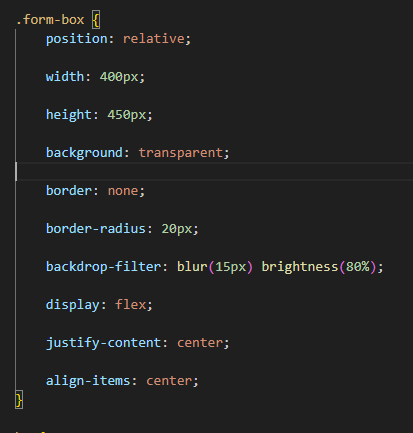
\includegraphics[width=13cm,height=6.7cm]{images/capture css.png}%
    }
    \caption{Code CSS pour styliser une zone dans la page de connection}%
\end{figure}

\subsection{JavScript}
JavaScript a été initialement créé pour “rendre les pages web vivantes”.
Les programmes dans ce langage sont appelés scripts. Ils peuvent être écrits directement dans une page HTML et exécutés automatiquement au chargement des pages. \cite{infojs}\par 

Nous avons également fait usage de jQuery qui est une bibliothèque JavaScript rapide, légère et riche en fonctionnalités\cite{jqueryinfo} . pour pouvoir gérer la fonctionnalité de recherche(filtre).


\subsection{PHP}
PHP (officiellement, ce sigle est un acronyme récursif pour PHP Hypertext Preprocessor) est un langage de scripts généraliste et Open Source, spécialement conçu pour le développement d'applications web. Il peut être intégré facilement au HTML.
Le grand avantage de PHP est qu'il est extrêmement simple pour les néophytes, mais offre des fonctionnalités avancées pour les experts\cite{infoPHP}.
La logique de notre plateforme a été codé en php à travers son framework Laravel.

 \begin{figure}[H]%
    \center%
    \setlength{\fboxsep}{5pt}%
    \setlength{\fboxrule}{0.5pt}%
    \fbox{
    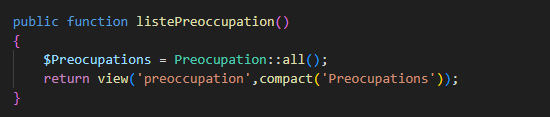
\includegraphics[width=13cm,height=6.7cm]{images/controllerpreoc.PNG}%
    }
    \caption{Code PHP pour la récupération des préoccupation en base de données}%
\end{figure}

\subsection{Framework Laravel}

\begin{figure}[H]%
    \center%
    \setlength{\fboxsep}{5pt}%
    \setlength{\fboxrule}{0.5pt}%
    \fbox{
    
\includegraphics[width=5cm,height=5cm]{images/laravel logo.png}%
    }
    \caption{Logo Laravel}%
\end{figure}

  Un framework web est un ensemble d'élément préétablie qui fournit une structure et un point de départ pour créer une application web, vous permettant ainsi de se concentrer sur la création de quelque chose d'extraordinaire au lieu des détails.
Laravel est un framework d'applications web avec une syntaxe expressive et élégante\cite{laravelinfo}.
\newpage
\subsection{SGBD MySQL}
\begin{figure}[H]%
    \center%
    \setlength{\fboxsep}{5pt}%
    \setlength{\fboxrule}{0.5pt}%
    \fbox{
    
\includegraphics[width=5cm,height=5cm]{images/logo mysql.png}%
    }
    \caption{Logo MySQL}%
\end{figure}
Pour la gestion des données, nous avons opté pour MySQL, offrant une solution robuste et fiable pour \index{stocker}stocker et récupérer les informations nécessaires à notre plateforme. Grâce au systeme de mapage eloquent de Laravel nous sommes parvenus à mettre en place  les différents systèmes de manipulation des données.

\section*{Conclusion}
Pour réaliser notre plateforme, nous avons en prélude fais le choix des outils et technologies nécessaire à cette réalisation. Nos différents chois ce sont basés sur des critères pertinent de sorte à être à l'aise tout au long de cette aventure. Nous avons opté pour le volet technologie pour VS code comme IDE, Git combiné a GitHub pour la \index{sauvegarde}sauvegarde et la méthodologie agile scrum. Pour le volet technologie nous avons choisi bien sur HTML, CSS et JavaScript pour réaliser nos interface et PHP avec son framework Laravel pour mettre en place la logique de notre plateforme. Le SGBD qui nous a semblé plus propice et pour le quel nous avons opté est MySQL. Tous ces outils et technologie nous on permis d'atteindre nos objectifs même si nous avons rencontré quelques soucis.%  Implementation et concretisation
     
       \chapter{Presentation de la plateforme}
\markboth{Chapitre 5. Présentation de la plateforme}{} 
\begin{spacing}{1.2}
\minitoc
\thispagestyle{MyStyle}
\end{spacing}
\newpage

\section*{Introduction}
Ce chapitre est dédié à la présentation de notre plateforme numérique, conçue pour centraliser et faciliter l'accès aux mémoires de thèse et mémoires de master. \par
 Après avoir surmonté les défis de l'accès limité et de la disponibilité restreinte des ressources dans les \index{bibliothèques physiques}, nous avons développé une solution innovante qui répond aux besoins de la communauté universitaire.
 Notre solution a été baptisé \textbf{Bibliothèse.UNZ} et compte 8 pages composée de différentes sections. 


\begin{figure}[H]%
    \center%
    \setlength{\fboxsep}{5pt}%
    \setlength{\fboxrule}{0.5pt}%
    \fbox{
    
\includegraphics[width=5cm,height=5cm]{images/logo btz.png}%
    }
    \caption{Logo de la plateforme}%
\end{figure}

\section{Quelques interfaces de la plateforme numérique des mémoires de thèse et de master}
Dans les sections suivantes, nous présenterons quelques interfaces utilisateur essentiel.

\subsection{Page d'accueil}
La première page de notre plateforme est composé de trois sections

\textbf{Section 1 :}
La toute première section qui est composé de deux carrousselles avec des images d'illustration.
\begin{figure}[H]%
    \center%
    \setlength{\fboxsep}{5pt}%
    \setlength{\fboxrule}{0.5pt}%
    \fbox{
    
\includegraphics[width=16cm,height=9cm]{images/p1s1.PNG}%
    }
    \caption{Première section de la page d'accueil}%
\end{figure}
\par 

\textbf{Section 2 :}
Cette section présente le nombre de ressources que nous avons dans chaque UFR et des boutons pour pouvoirs consulter chaque catalogue.

\begin{figure}[H]%
    \center%
    \setlength{\fboxsep}{5pt}%
    \setlength{\fboxrule}{0.5pt}%
    \fbox{
    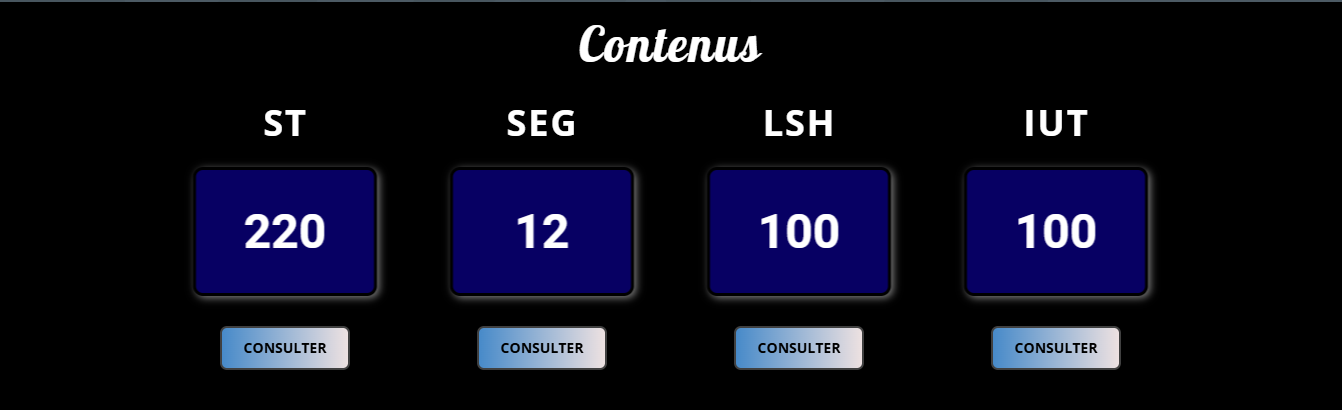
\includegraphics[width=16cm,height=9cm]{images/p1s2.PNG}%
    }
    \caption{Section pour le nombre de ressources disponible par UFR sur la plateforme }%
\end{figure}
\par

\textbf{Section 3 :}
A la troisième section nous avons les différents enseignants encadreur. Elle a pour but de permettre une meilleur indication concernant les noms des encadreurs figurant sur les travaux

\begin{figure}[H]%
    \center%
    \setlength{\fboxsep}{5pt}%
    \setlength{\fboxrule}{0.5pt}%
    \fbox{
    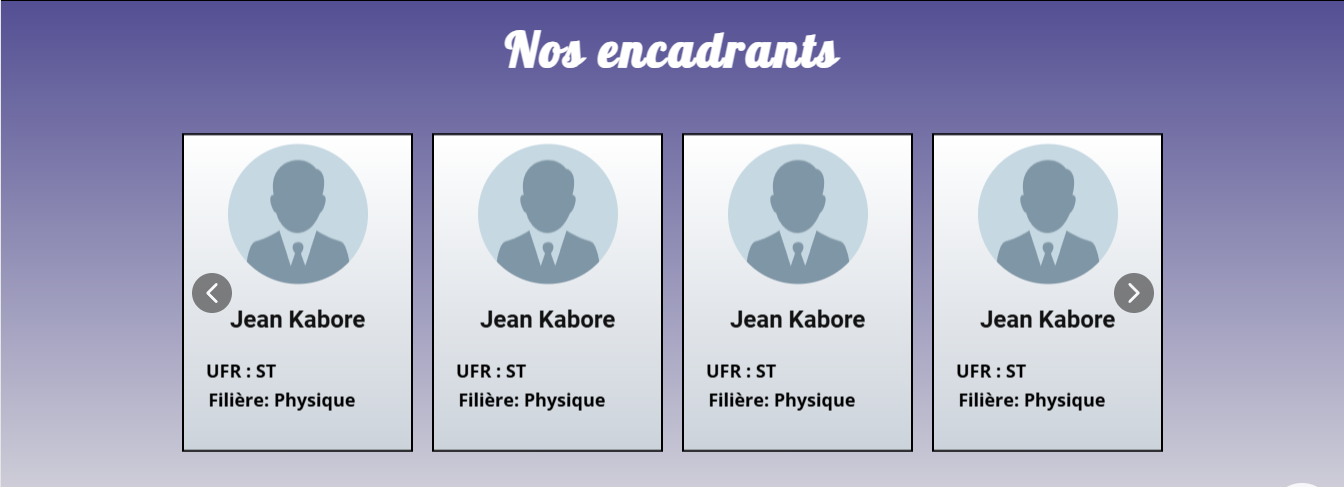
\includegraphics[width=16cm,height=9cm]{images/p1S3.PNG}%
    }
    \caption{Section pour les encadrants}%
\end{figure}
\par


\subsection{Liste des ressources}
Cette page présente la liste de ressources pour la catégorie sélectionné.

\begin{figure}[H]%
    \center%
    \setlength{\fboxsep}{5pt}%
    \setlength{\fboxrule}{0.5pt}%
    \fbox{
    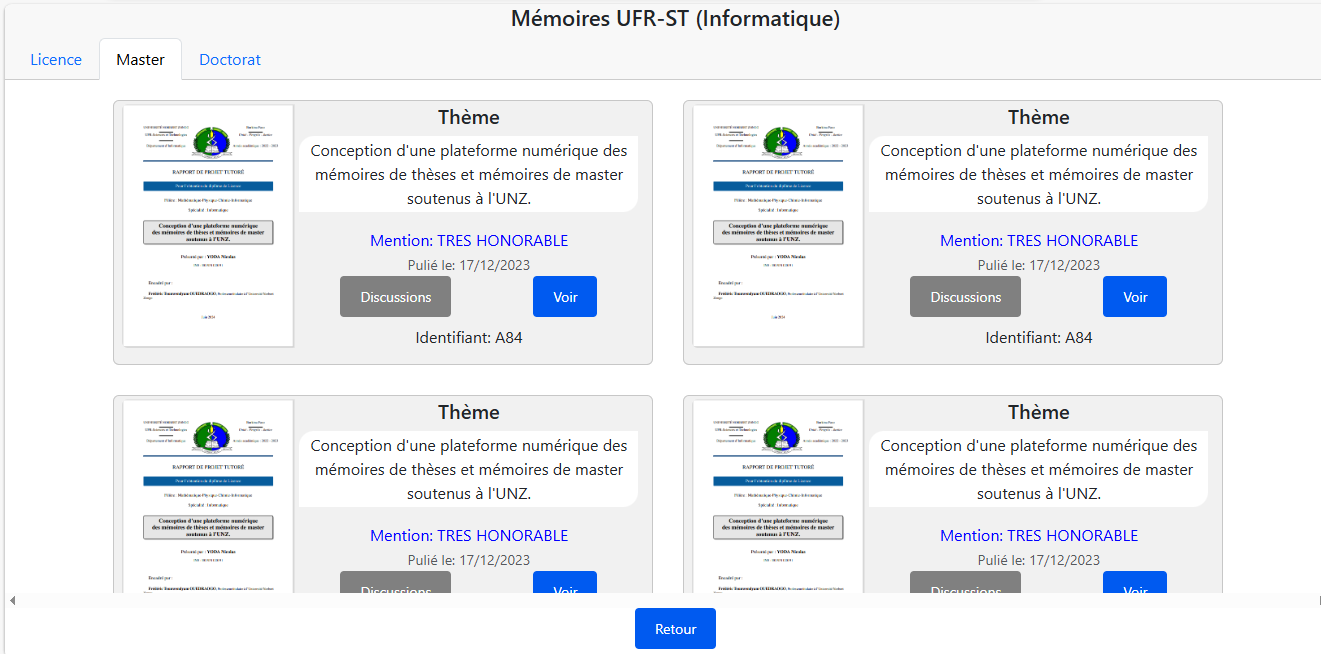
\includegraphics[width=16cm,height=9cm]{images/ressources.PNG}%
    }
    \caption{Liste des ressources}%
\end{figure}

\subsection{Formulaire de préoccupation}
Cette page présente le formulaire permettant aux utilisateurs de saisir leur préoccupation.

\begin{figure}[H]%
    \center%
    \setlength{\fboxsep}{5pt}%
    \setlength{\fboxrule}{0.5pt}%
    \fbox{
    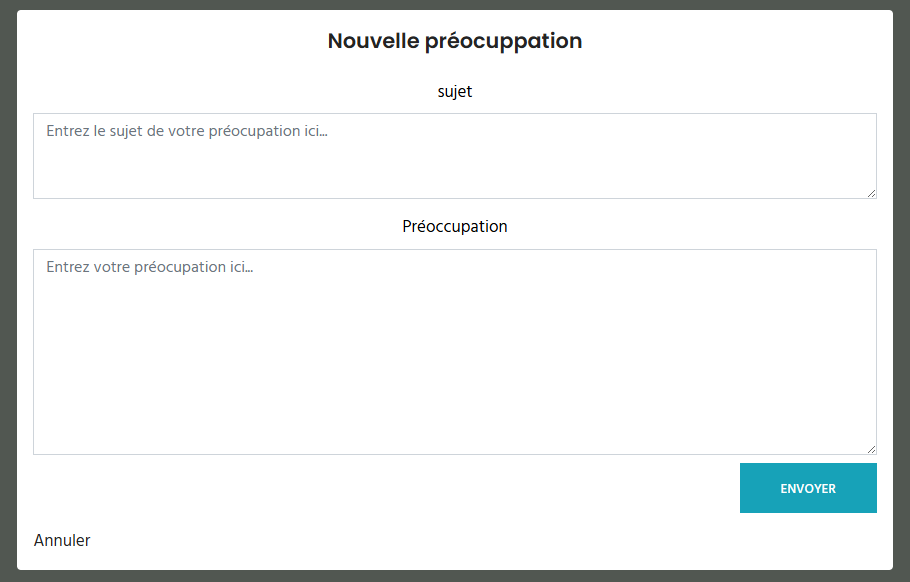
\includegraphics[width=16cm,height=9cm]{images/preocupation.PNG}%
    }
    \caption{Formulaire des préoccupations}%
\end{figure}

\subsection{Liste des préoccupations}
Ici nou avons la liste des différentes préoccupation qui ont été posé et un lien menant à la discussion concernant chaque préoccupation.

\begin{figure}[H]%
    \center%
    \setlength{\fboxsep}{5pt}%
    \setlength{\fboxrule}{0.5pt}%
    \fbox{
    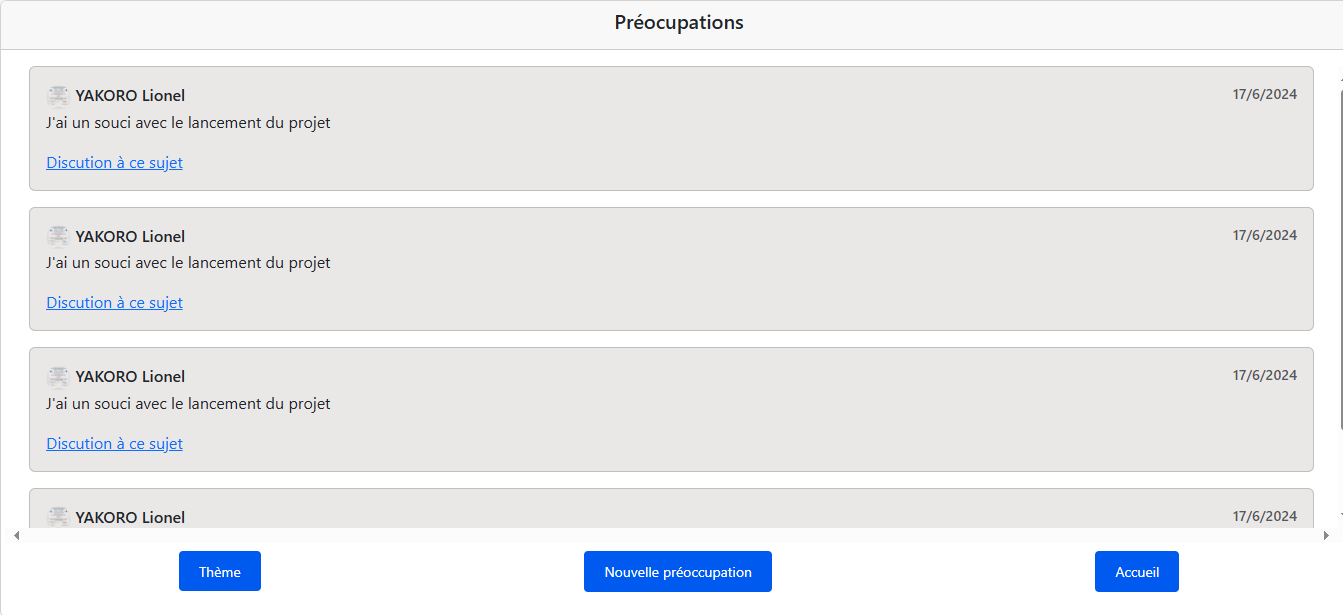
\includegraphics[width=16cm,height=9cm]{images/liste des preocupation.PNG}%
    }
    \caption{Liste des préoccupations}%
\end{figure}

\subsection*{Conclusion}
En conclusion nous pouvons affirmer que les différentes étapes de notre aventure nous ont permis de mettre en place une plateforme de 8 principales pages dénommée Bibliothèse.UNZ capable de stocker en ligne les mémoires de thèses et mémoires de master au format PDF et qui dispose de fonctionnalité de recherche ainsi qu'un cadre d'échange collaboratif entre les membres de la communauté universitaire.%Prsentation de la plateforme
     
     vc\chapter{Analyse et discussion des résultats}
\markboth{Chapitre 6. Analyse et discussion des résultats}{} 
\begin{spacing}{1.2}
\minitoc
\thispagestyle{MyStyle}
\end{spacing}
\newpage

\section*{Introduction}
Dans cette section, nous analysons et discutons les résultats obtenus lors de la mise en œuvre de notre plateforme numérique pour la gestion et l'accès aux thèses et mémoires. Cette analyse permettra d'évaluer dans quelle mesure les objectifs du projet ont été atteints et d'identifier les forces et les faiblesses de notre approche.

\section{Analyse des résultats}
\subsubsection{Accessibilité de la plateforme}
\textbf{Observation :} La plateforme permet un accès centralisé et en ligne aux thèses et mémoires, accessible depuis un ordinateur ou un smartphone connecté à internet.\par

\textbf{Analyse :} L'utilisation du langage de balisage HTML et du CSS a permis de créer une interface utilisateur intuitive et responsive, facilitant la navigation et la recherche de documents. Les fonctionnalités de recherche avancée intégrées via JavaScript et jQuery ont considérablement amélioré l'expérience utilisateur en permettant des filtres et des requêtes rapides.

\subsection{Gestion des données et performances}
\textbf{Observation :} L'intégration de MySQL et Eloquent ORM de Laravel a permis une gestion efficace des données, incluant des opérations CRUD rapides et sécurisées.\par

\textbf{Analyse :} L'utilisation de Laravel a simplifié la gestion des relations complexes entre les différentes entités de la base de données. Les requêtes optimisées ont contribué à de bonnes performances, même avec un nombre croissant de documents.

\subsection{Sécurité et fiabilité}
\textbf{Observation :} La plateforme intègre des mécanismes de sécurité robustes pour protéger les données et les utilisateurs. \par

\textbf{Analyse :} Grâce aux fonctionnalités de sécurité de Laravel, telles que l'authentification et l'autorisation des utilisateurs, la plateforme garantit un accès sécurisé aux données. Les sauvegardes régulières et la protection contre les injections SQL renforcent la fiabilité de l'application.

\section{Discussion}

\subsection{Avantages et Réalisations}
\renewcommand{\labelitemi}{\tiny$\bullet$}
\begin{itemize}[leftmargin=2cm, topsep=0pt]
        \begin{spacing}{1.25}
        \item \textbf{Accessibilité :}
        La numérisation des thèses et mémoires a supprimé les barrières géographiques, permettant un accès global et simultané à des documents précieux.
      \item \textbf{Efficacité de recherche :}
        Les fonctionnalités de recherche avancée ont réduit le temps nécessaire pour localiser des documents pertinents, améliorant ainsi l'efficacité académique.
        
        \item \textbf{Interaction et collaboration :} L'interface utilisateur interactive favorise les échanges entre les membres de la communauté universitaire, enrichissant les discussions académiques et la compréhension des travaux.
        \end{spacing}
\end{itemize}

\subsection{Limites et défis}
\renewcommand{\labelitemi}{\tiny$\bullet$}
\begin{itemize}[leftmargin=2cm, topsep=0pt]
        \begin{spacing}{1.25}
        \item \textbf{Adoption et formation :}
        Bien que la plateforme soit simple d'utilisation et techniquement solide, l'adoption par tous les utilisateurs peut nécessiter des efforts supplémentaires en termes de formation et de support.
        
         \item \textbf{Connectivité  :}
         Une connexion Internet est nécessaire pour accéder aux documents non téléchargé et aux interactions, ce qui peut être problématique dans les zones avec une connectivité limitée ou inexistante.
        
         \item \textbf{Temps de chargement :} La vitesse d'accès peut être affectée par une connexion Internet lente, rendant l'expérience utilisateur moins fluide.
        
        \item \textbf{Compatibilité des formats :} L'intégration de formats de documents autre que le PDF n'est pas pris en compte.
        
        \end{spacing}
\end{itemize}

\subsection{Perspectives}
\renewcommand{\labelitemi}{\tiny$\bullet$}
\begin{itemize}[leftmargin=2cm, topsep=0pt]
        \begin{spacing}{1.25}
        \item \textbf{Amélioration de l'interface :}
        Des itérations futures pourraient se concentrer sur l'amélioration continue de l'interface utilisateur, en intégrant des retours d'expérience et en optimisant l'ergonomie.
        
      \item \textbf{Fonctionnalités avancées  :}
        L'ajout de fonctionnalités telles que la recommandation de documents basée sur l'intelligence artificielle ou des outils de collaboration en temps réel pourrait enrichir davantage la plateforme.
        
        \item \textbf{Intégration mobile :}Développer des applications mobiles dédiées pourrait accroître l'accessibilité et l'utilisation de la plateforme.
        \end{spacing}
\end{itemize}

%Analyse et discussion des resultats
     
    \chapter*{CONCLUSION GENERALE}
\markboth{\MakeUppercase{CONCLUSION GENERALE}}{}
\addcontentsline{toc}{chapter}{CONCLUSION GENERALE}
\adjustmtc
\thispagestyle{MyStyle}


La réalisation de notre plateforme numérique des mémoires de thèse et mémoires de master marque une étape significative dans la facilitation de l'accès aux ressources académiques. Confrontés aux nombreuses limitations des bibliothèques physiques, telles que la disponibilité restreinte des documents, le nombre limité de copies et la difficulté à localiser des thèses et mémoires de qualité, nous avons développé une plateforme innovante pour centraliser et faciliter l'accès aux documents académiques.

Notre projet s'est structuré autour de plusieurs étapes clés, allant de la conception à la mise en œuvre. Nous avons minutieusement choisi des technologies appropriées pour répondre aux besoins spécifiques de notre plateforme. HTML et CSS ont été utilisés pour créer une interface utilisateur intuitive et responsive, tandis que PHP avec le framework Laravel et JavaScript avec la bibliothèque jQuery ont fourni la robustesse nécessaire pour les fonctionnalités de backend et d'interactivité. De plus, l'utilisation de MySQL a permis une gestion efficace et sécurisée des données.

Tout au long du développement, nous avons rencontré et surmonté divers défis techniques et conceptuels. L'intégration de ces technologies a non seulement amélioré l'accessibilité des documents, mais a également optimisé l'expérience utilisateur en offrant des fonctionnalités de recherche avancée et une interface conviviale.

Les résultats obtenus démontrent que notre plateforme numérique des mémoires de thèse et mémoires de master répond aux besoins pressants dede la communauté universitaire en offrant un accès simplifié, sécurisé et simultané aux ressources académiques, indépendamment des contraintes géographiques. Notre plateforme permet une recherche rapide et précise des documents, ce qui facilite grandement le travail académique et la recherche.

Cependant, la mise en place de cette plateforme numérique n'est qu'une première étape. Il reste des défis à relever, notamment en termes d'optimisation continue de la plateforme, de l'ajout de nouvelles fonctionnalités et de l'amélioration de l'expérience utilisateur. Il y a également l'intégration d'applications mobiles et l'utilisation de l'intelligence artificielle pour enrichir encore plus les fonctionnalités de recherche et personnaliser l'expérience utilisateur.

Grosso modo, notre plateforme numérique représente une avancée majeure dans l'accès aux ressources académiques. Elle répond de manière efficace aux défis posés par les bibliothèques physiques et offre une solution innovante pour la gestion et la diffusion des connaissances. Nous espérons que cette plateforme contribuera significativement à l'avancement de la recherche et de l'éducation, en favorisant un accès ouvert et collaboratif aux savoirs académiques. Par cette initiative, nous nous engageons à promouvoir une culture de partage et d'innovation, au bénéfice de toute la communauté académique.\par




\newpage
\addtocontents{toc}{\protect\thispagestyle{MyStyle}} % Appliquer le style de page personnalisé

% Générer la liste des termes indexés avec un interligne simple
\begin{spacing}{1}
    \printindex % Imprimer l'index
\end{spacing}

\renewcommand{\indexname}{LISTE DES TERMES INDEXES} 
% Ajouter la liste des termes indexés à la table des matières
\addcontentsline{toc}{chapter}{\indexname}

    %@book{loeliger2012version,
  title={Version Control with Git: Powerful tools and techniques for collaborative software development},
  author={Loeliger, Jon and McCullough, Matthew},
  year={2012},
  publisher={" O'Reilly Media, Inc."},
  pages={1--6}
}
@article{schwaber2011scrum,
  title={The scrum guide},
  author={Schwaber, Ken and Sutherland, Jeff},
  journal={Scrum Alliance},
  volume={21},
  number={1},
  pages={1--7},
  year={2011}
}

\addcontentsline{toc}{chapter}{BIBLIOGRAPHIE}
\adjustmtc
\renewcommand\bibname{BIBLIOGRAPHIE}
\begin{thebibliography}{25}
\thispagestyle{MyStyle}

@article{schwaber2011scrum,
  title={The scrum guide},
  author={Schwaber, Ken and Sutherland, Jeff},
  journal={Scrum Alliance},
  volume={21},
  number={1},
  pages={1--7},
  year={2011}
}


@book{loeliger2012version,
  title={Version Control with Git: Powerful tools and techniques for collaborative software development},
  author={Loeliger, Jon and McCullough, Matthew},
  year={2012},
  publisher={" O'Reilly Media, Inc."},
  pages={1--6}
}
\end{thebibliography} 


   \bibliographystyle{unsrt}
  % Style de la bibliographie
\bibliography{bibliographie}%  Nom du fichier .bib (sans l'extension)

    %\chapter*{ANNEXES}
\markboth{\MakeUppercase{ANNEXES}}{}
\addcontentsline{toc}{chapter}{ANNEXES}
\adjustmtc
\thispagestyle{MyStyle}

%% add to table of contents : Annexe.1
\makeatletter\renewcommand\thesection{A.\@arabic\c@section}\makeatother

%add spacing in the table of figures
\addtocontents{lof}{\vspace{0.3cm}}

\appendix
\renewcommand{\thefigure}{A.\arabic{figure}}
\setcounter{figure}{0}
\section{TITRE ANNEXE 1}
Lorem ipsum dolor sit amet, consectetur adipiscing elit. Sed non risus. Suspendisse lectus tortor, dignissim sit amet, adipiscing nec, ultricies sed, dolor. Cras elementum ultrices diam. Maecenas ligula massa, varius a, semper congue, euismod non, mi. Proin porttitor, orci nec nonummy molestie, enim est eleifend mi, non fermentum diam nisl sit amet erat. Duis semper. Duis arcu massa, scelerisque vitae, consequat in, pretium a, enim.\par
\begin{figure}[H]%
    \center%
    \setlength{\fboxsep}{5pt}%
    \setlength{\fboxrule}{0.5pt}%
    \fbox{
    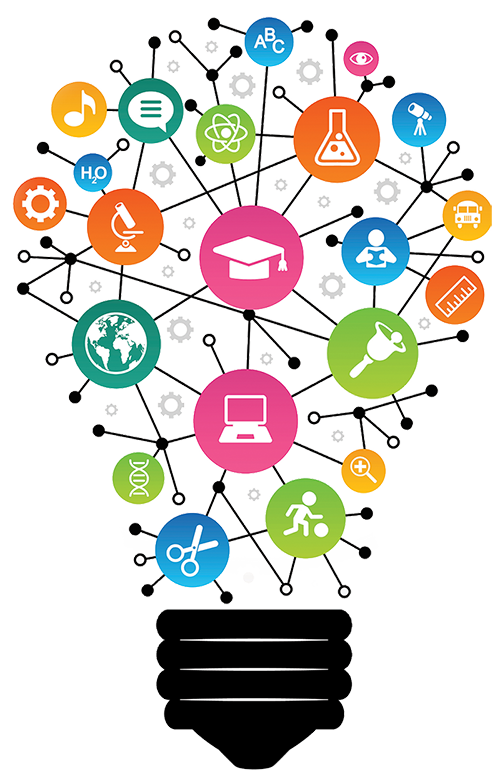
\includegraphics[width=6.5cm,height=9cm]{images/your_image.png}%
    }
    \caption{Titre de figure annexe 1}%
\end{figure}

\section{TITRE ANNEXE 2}
Lorem ipsum dolor sit amet, consectetur adipiscing elit. Sed non risus. Suspendisse lectus tortor, dignissim sit amet, adipiscing nec, ultricies sed, dolor. Cras elementum ultrices diam. Maecenas ligula massa, varius a, semper congue, euismod non, mi. Proin porttitor, orci nec nonummy molestie, enim est eleifend mi, non fermentum diam nisl sit amet erat. Duis semper. Duis arcu massa, scelerisque vitae, consequat in, pretium a, enim. Pellentesque congue. Ut in risus volutpat libero pharetra tempor.\par
\begin{figure}[H]%
    \center%
    \setlength{\fboxsep}{5pt}%
    \setlength{\fboxrule}{0.5pt}%
    \fbox{
    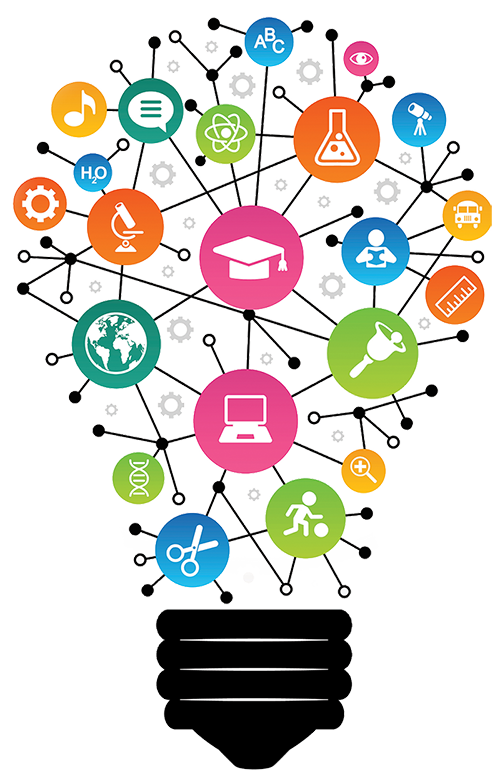
\includegraphics[width=6.5cm,height=9cm]{images/your_image.png}%
    }
    \caption{Titre de figure annexe 2}%
\end{figure}

    
    \newpage
\thispagestyle{empty}
\begin{center}
  \renewcommand*{\familydefault}{\defaultFont}
  \fontsize{12pt}{12pt}\selectfont%
  \textbf{
  Conception d'une plateforme numérique\\des mémoires de thèses et mémoires de master soutenus à l'UNZ\\%
  }
\vspace{15pt} {%
  \begin{spacing}{0.05}
    \rule{200pt}{2pt}\\
    \rule{200pt}{0.75pt}\\
  \end{spacing}
  \renewcommand*{\familydefault}{\defaultFont}
  \fontsize{14pt}{14pt}\selectfont%
  \vspace{15pt}
  \textbf{Nicolas YODA}
  \vspace{8pt}
  \begin{spacing}{0.05}
    \rule{200pt}{0.75pt}\\
    \rule{200pt}{2pt}\\
  \end{spacing}
}
\end{center}

%Français
\fontsize{12pt}{12pt}\selectfont%
\underline{\textbf{Résumé:}}\\
La réalisation de notre bibliothèque numérique s'inscrit dans un contexte où l'accès aux ressources académiques dans les bibliothèques physiques présente de nombreux défis. Les limitations de disponibilité des documents, le nombre limité de copies, et la difficulté à localiser des thèses ou mémoires de qualité et pertinents sont autant de problématiques que nous avons cherché à surmonter. Cette plateforme vise à offrir une solution moderne et efficace pour centraliser et faciliter l'accès aux documents académiques.

Notre projet s'est structuré autour de plusieurs étapes clés, de la conception à la mise en œuvre. Dans ce mémoire, nous détaillons le processus de développement, en commençant par le choix des technologies appropriées. HTML et CSS ont été utilisés pour créer une interface utilisateur intuitive et responsive, tandis que PHP avec le framework Laravel et JavaScript avec la bibliothèque jQuery ont fourni la robustesse nécessaire pour les fonctionnalités de backend et d'interactivité.

\begin{spacing}{1}
\underline{\textbf{Mots clés:}}Backend, Framework, Responsive, Bibliothèque jQuery.\\
\end{spacing}


\underline{\textbf{Abstract :}}\\
The creation of our digital library addresses the challenges associated with accessing academic resources in physical libraries. Issues such as limited document availability, a restricted number of copies, and the difficulty in locating high-quality and relevant theses or dissertations were significant obstacles we aimed to overcome. This platform aims to offer a modern and efficient solution for centralizing and facilitating access to academic documents.

Our project followed several key stages, from design to implementation. In this thesis, we detail the development process, starting with the selection of appropriate technologies. HTML and CSS were used to create an intuitive and responsive user interface, while PHP with the Laravel framework and JavaScript with the jQuery library provided the necessary robustness for backend functionalities and interactivity.\par
\begin{spacing}{1}
\underline{\textbf{Key-words:}} backend, Framework, Responsive, jQuery library.\\
\end{spacing}



    

\end{document}